(a) From HW~\ref{hw:vtol}.\ref{chap:transfer_function_models}, the transfer function model is
\[
H(s) = \frac{\left(\frac{1}{m_c + 2 m_r}\right)}{s^2}\tilde{F}(s) = P_{lon}(s)\tilde{F}(s).
\]
Figure~\ref{fig:hw_vtol_lon_compensator_design_1} shows the Bode plot for $P_{lon}$ together with the design specification on tracking and attenuating the noise.  The requirement to reject constant input disturbances requires the inclusion of an integrator which is not shown in Figure~\ref{fig:hw_vtol_lon_compensator_design_1}.
%
\begin{figure}[H]
   \centering
   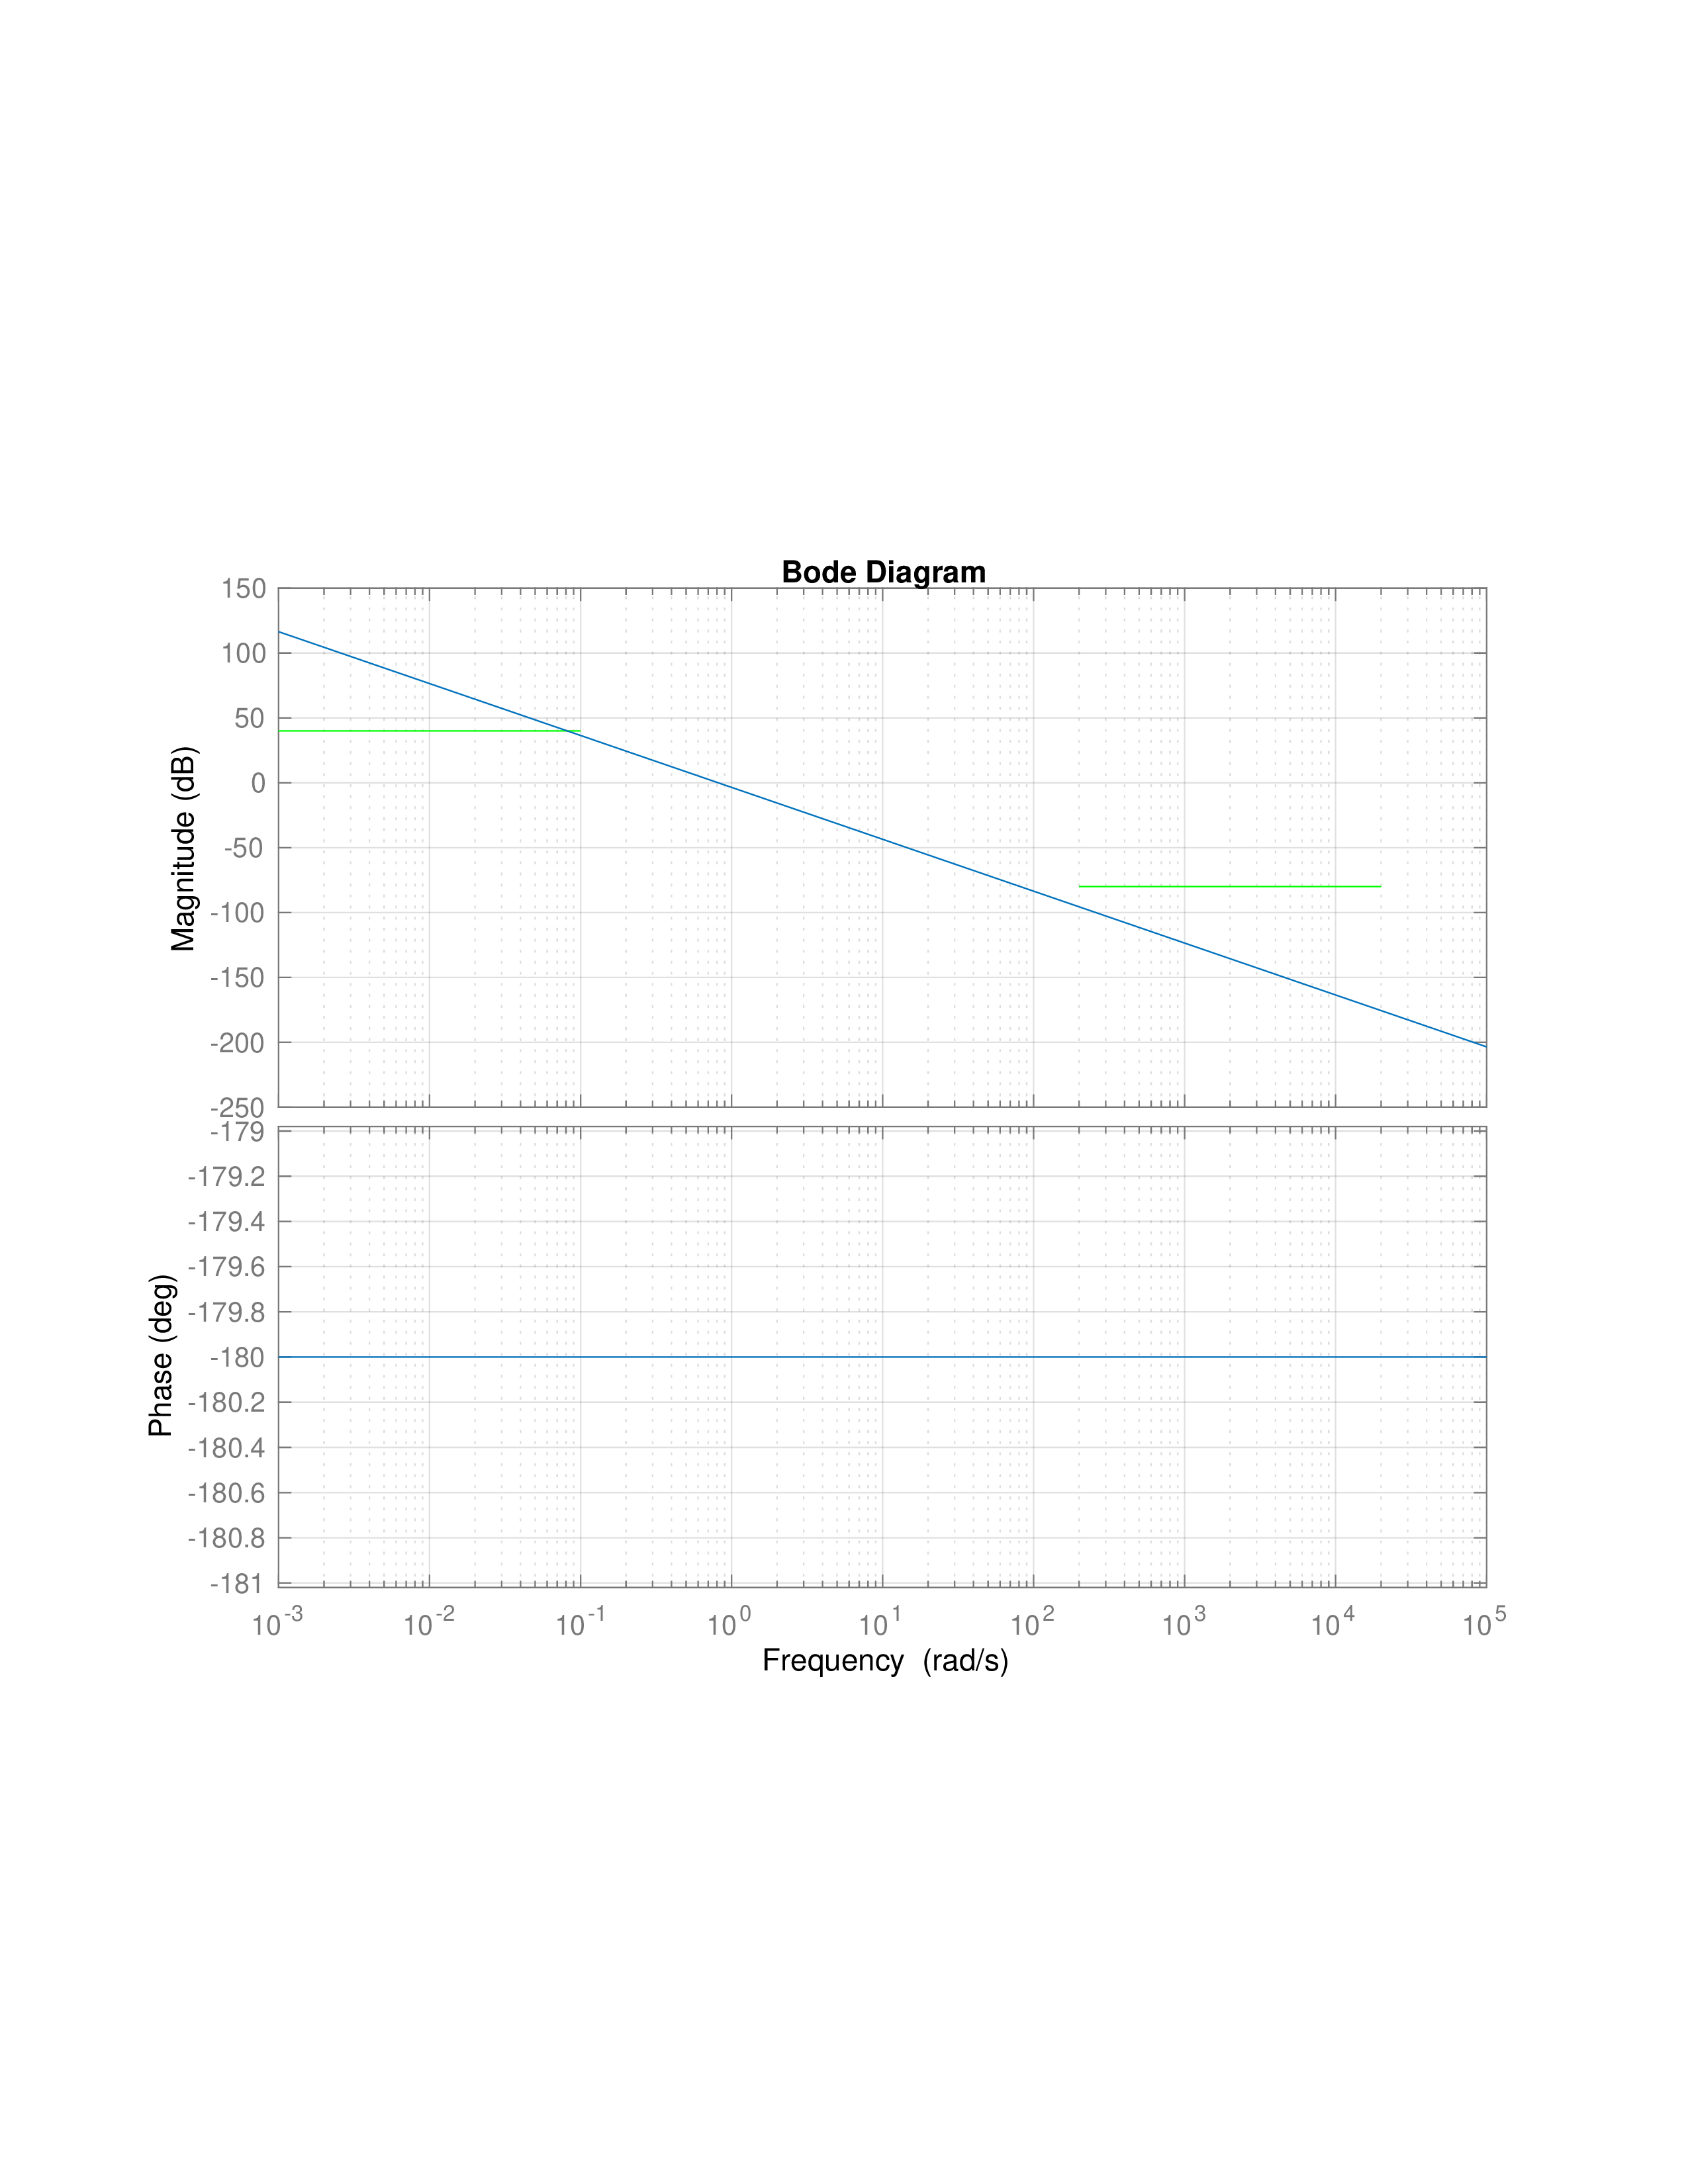
\includegraphics[width=0.95\textwidth]{6_design_studies/figures/hw_vtol_lon_compensator_design_1.pdf}
   \caption{The Bode plot for the plant in HW~\ref{hw:vtol}.\ref{chap:loopshaping_design}, together with the design specifications.}
   \label{fig:hw_vtol_lon_compensator_design_1}
\end{figure}

The first step is to add a phase lead element to stabilize the system.  Figure~\ref{fig:hw_vtol_lon_compensator_design_2} shows the loopgain with the addition of the phase lead filter
\[
C_{lead} = \frac{45(s+1/\sqrt{45})}{s+1/\sqrt{45}},
\]
and a proportional gain of $k_P=0.4$.
\begin{figure}[H]
   \centering
   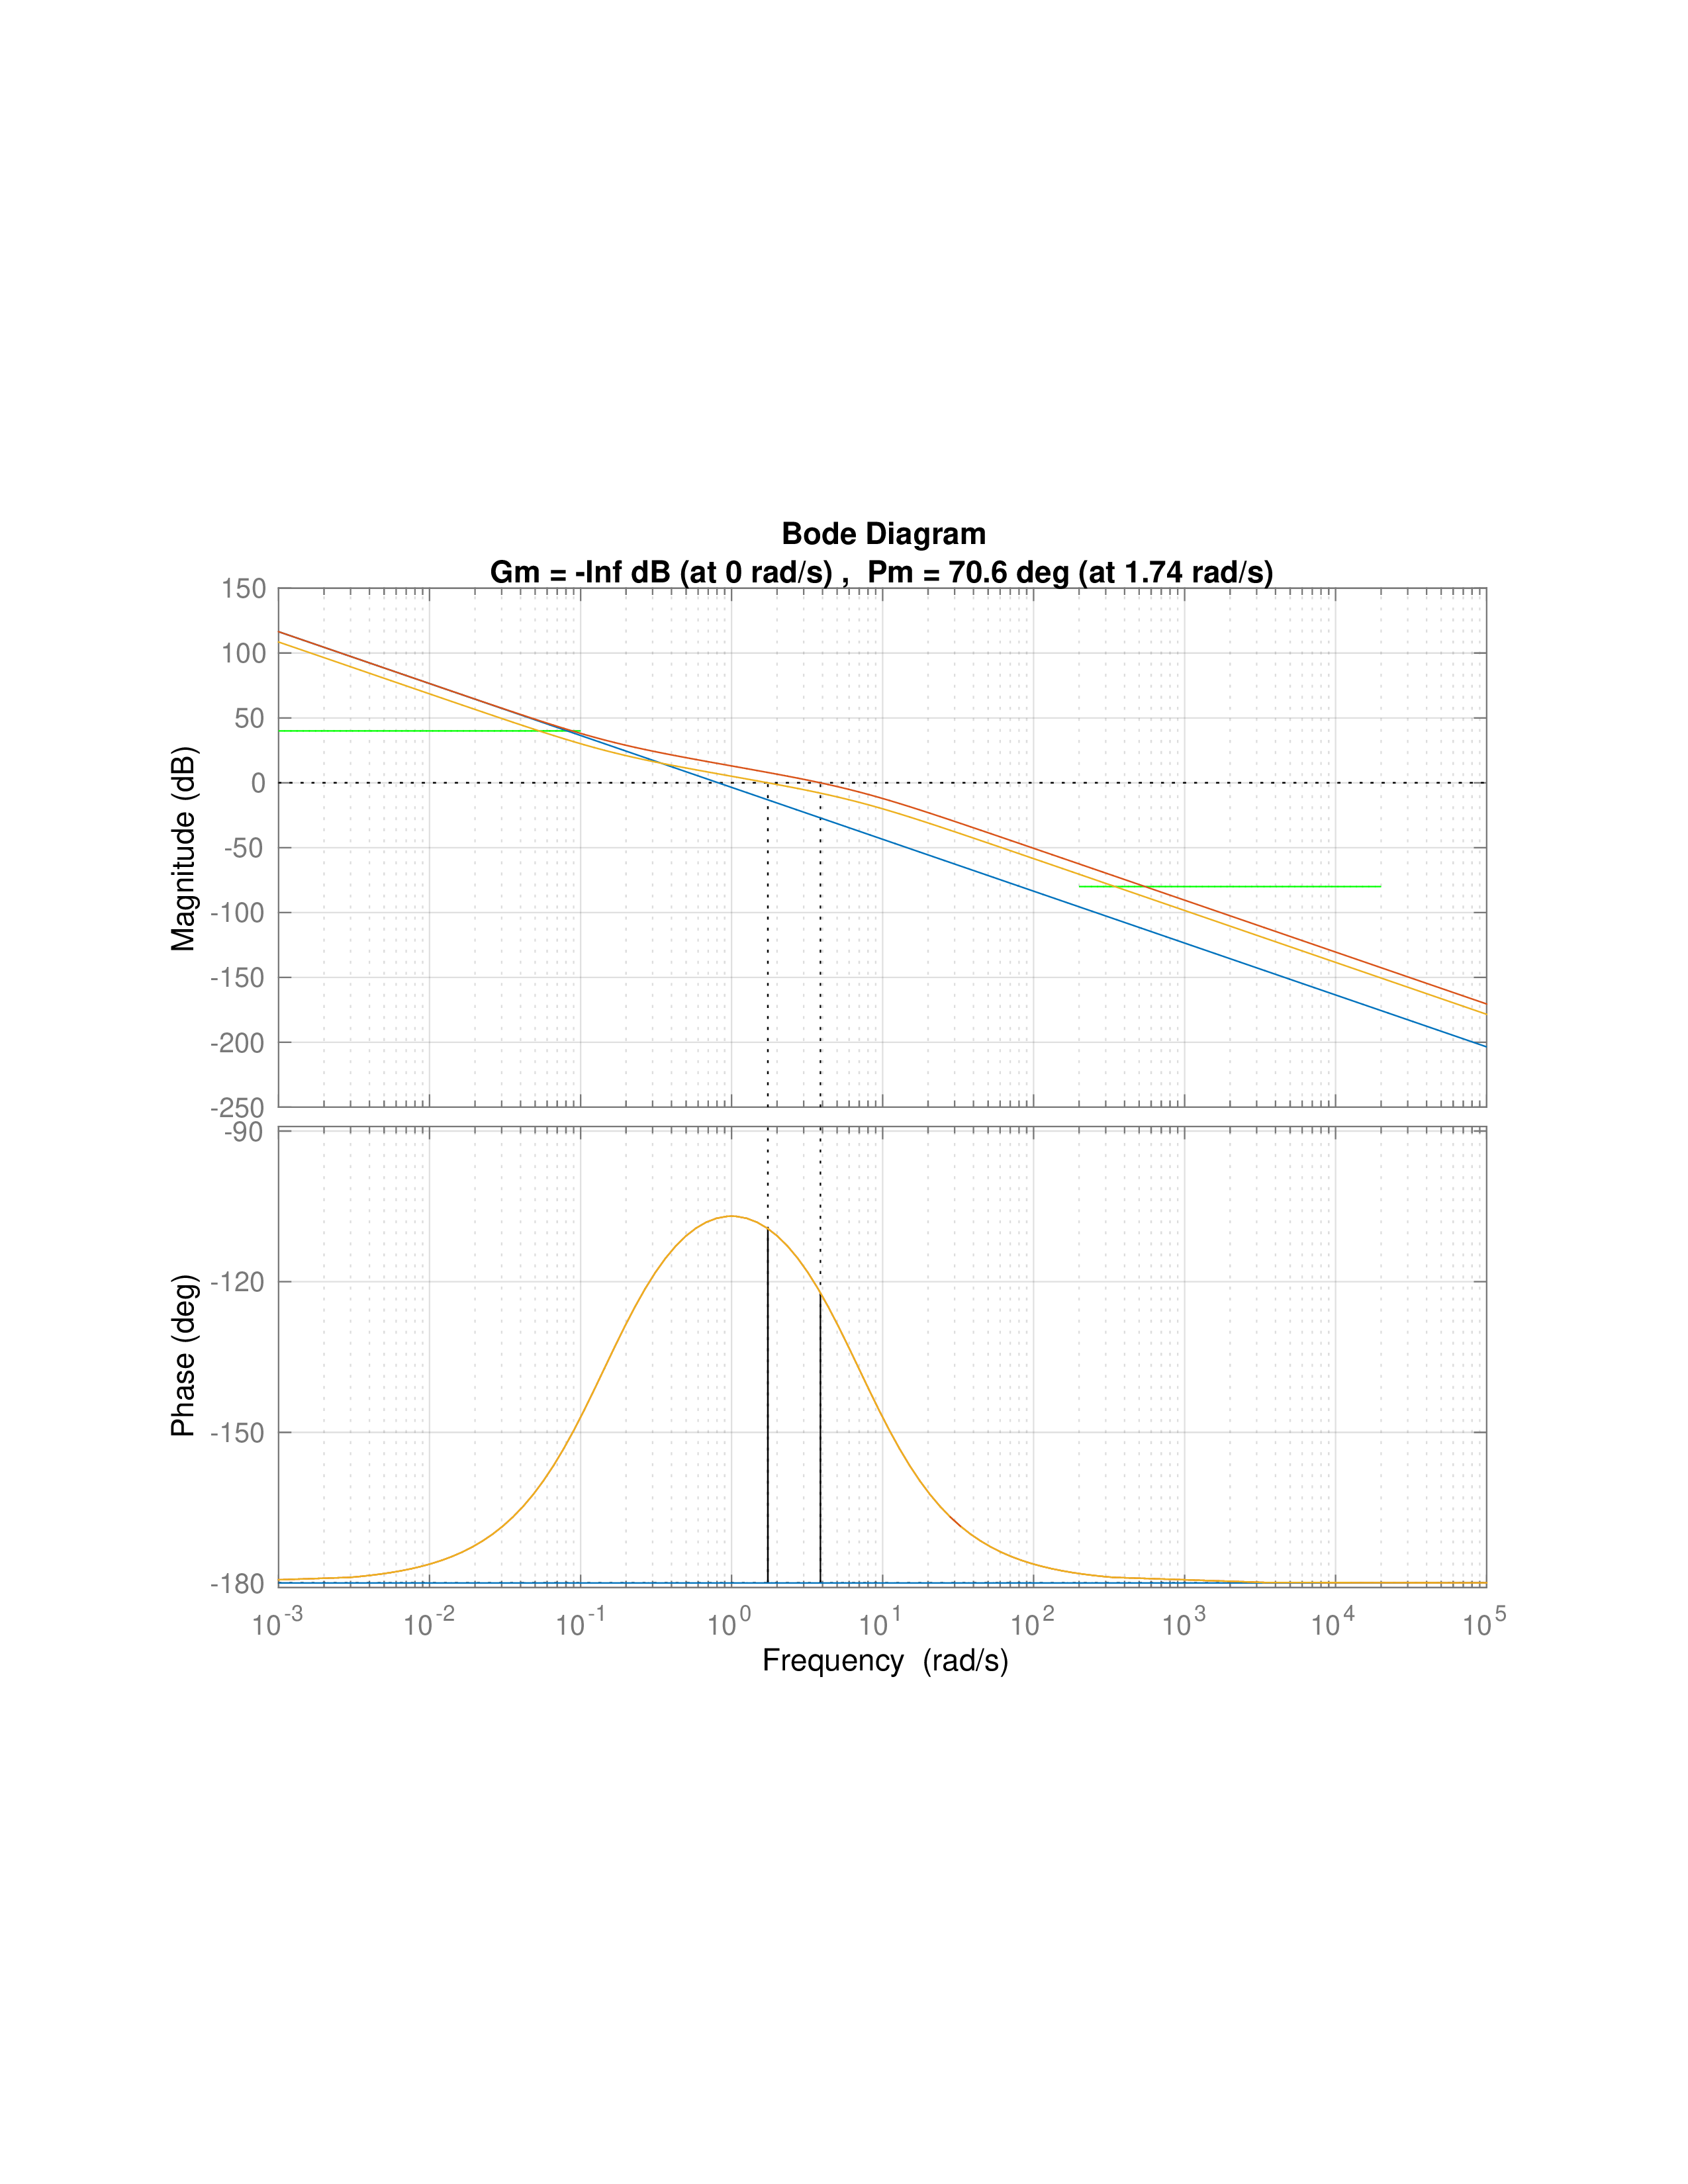
\includegraphics[width=0.95\textwidth]{6_design_studies/figures/hw_vtol_lon_compensator_design_2.pdf}
   \caption{The Bode plot for the system in HW~\ref{hw:vtol}.\ref{chap:loopshaping_design}, with phase lead, and proportional control.}
   \label{fig:hw_vtol_lon_compensator_design_2}
\end{figure}
To meet the requirement on rejecting input disturbances, an integrator is added, as shown in Figure~\ref{fig:hw_vtol_lon_compensator_design_3} where
\[
C_{int} = \frac{s+0.5}{s}.
\]
\begin{figure}[H]
   \centering
   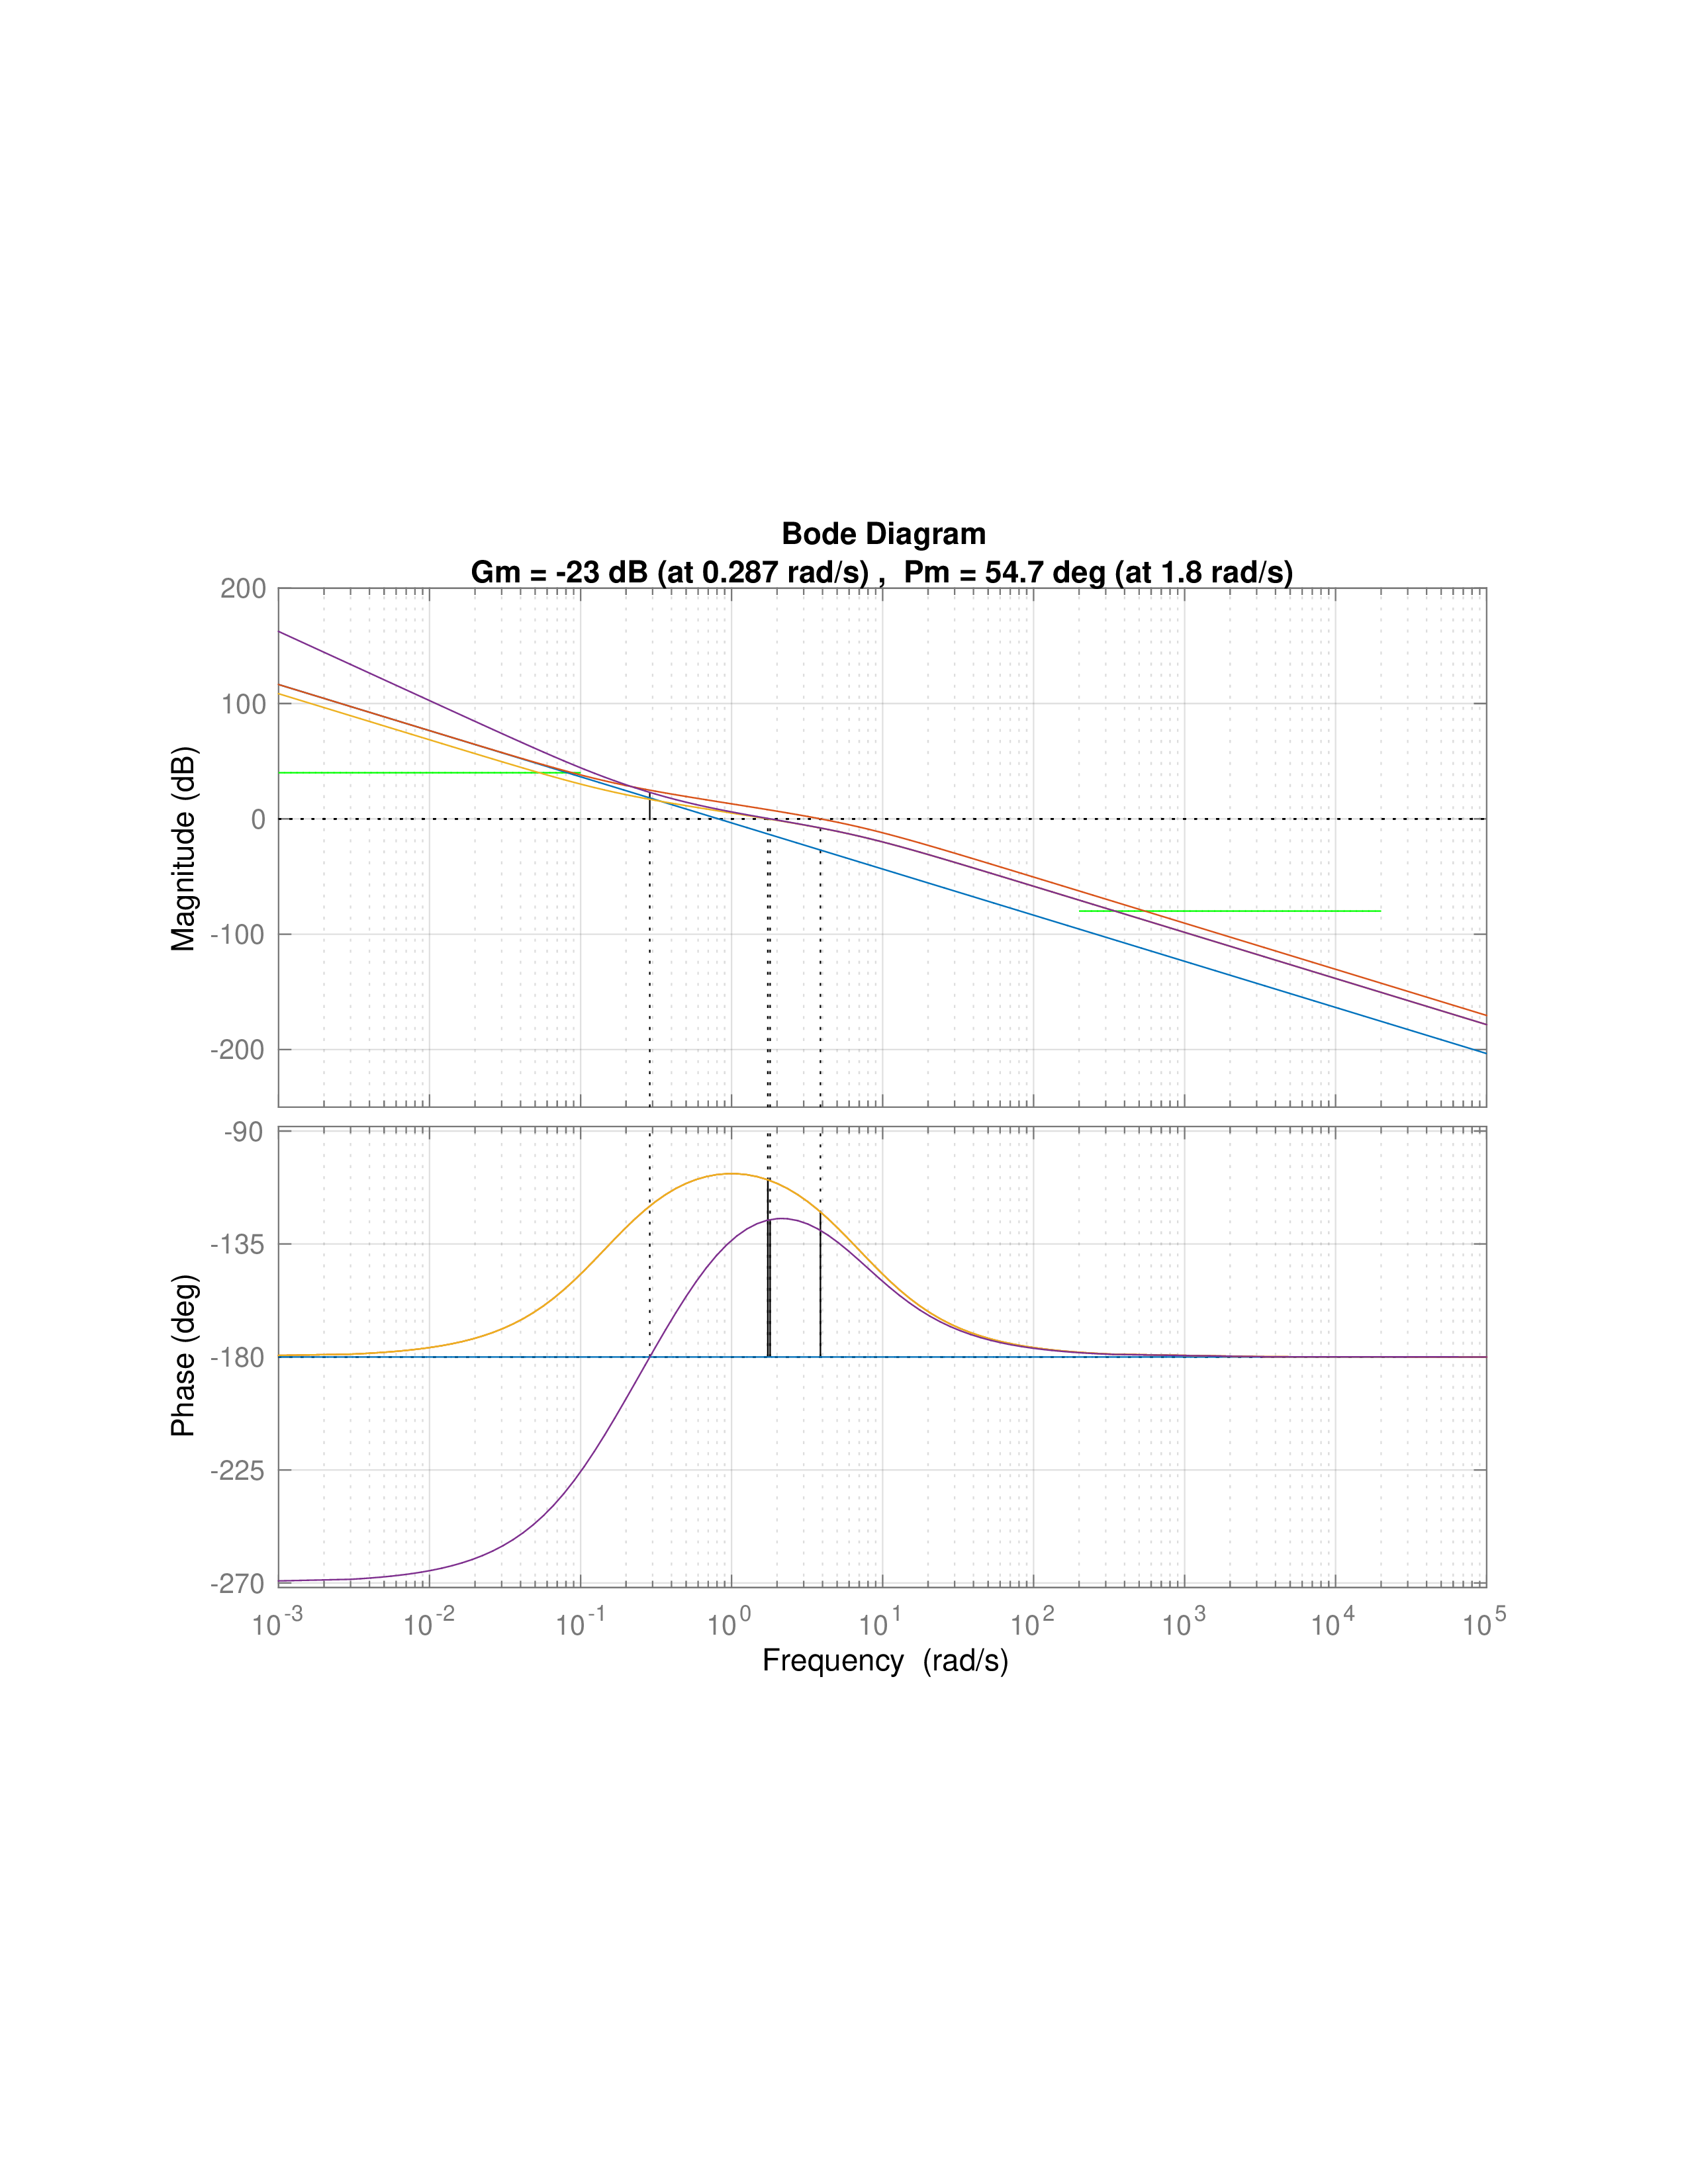
\includegraphics[width=0.95\textwidth]{6_design_studies/figures/hw_vtol_lon_compensator_design_3.pdf}
   \caption{The Bode plot for the outer loop system in HW~\ref{hw:vtol}.\ref{chap:loopshaping_design}, phase lead, proportional, andintegral control.}
   \label{fig:hw_vtol_lon_compensator_design_3}
\end{figure}
To meet the spec on noise attenuation, the low pass filter
\[
C_{lpf} = \frac{50}{s+50}
\]
and the result is shown in Figure~\ref{fig:hw_vtol_lon_compensator_design_4}.
\begin{figure}[H]
   \centering
   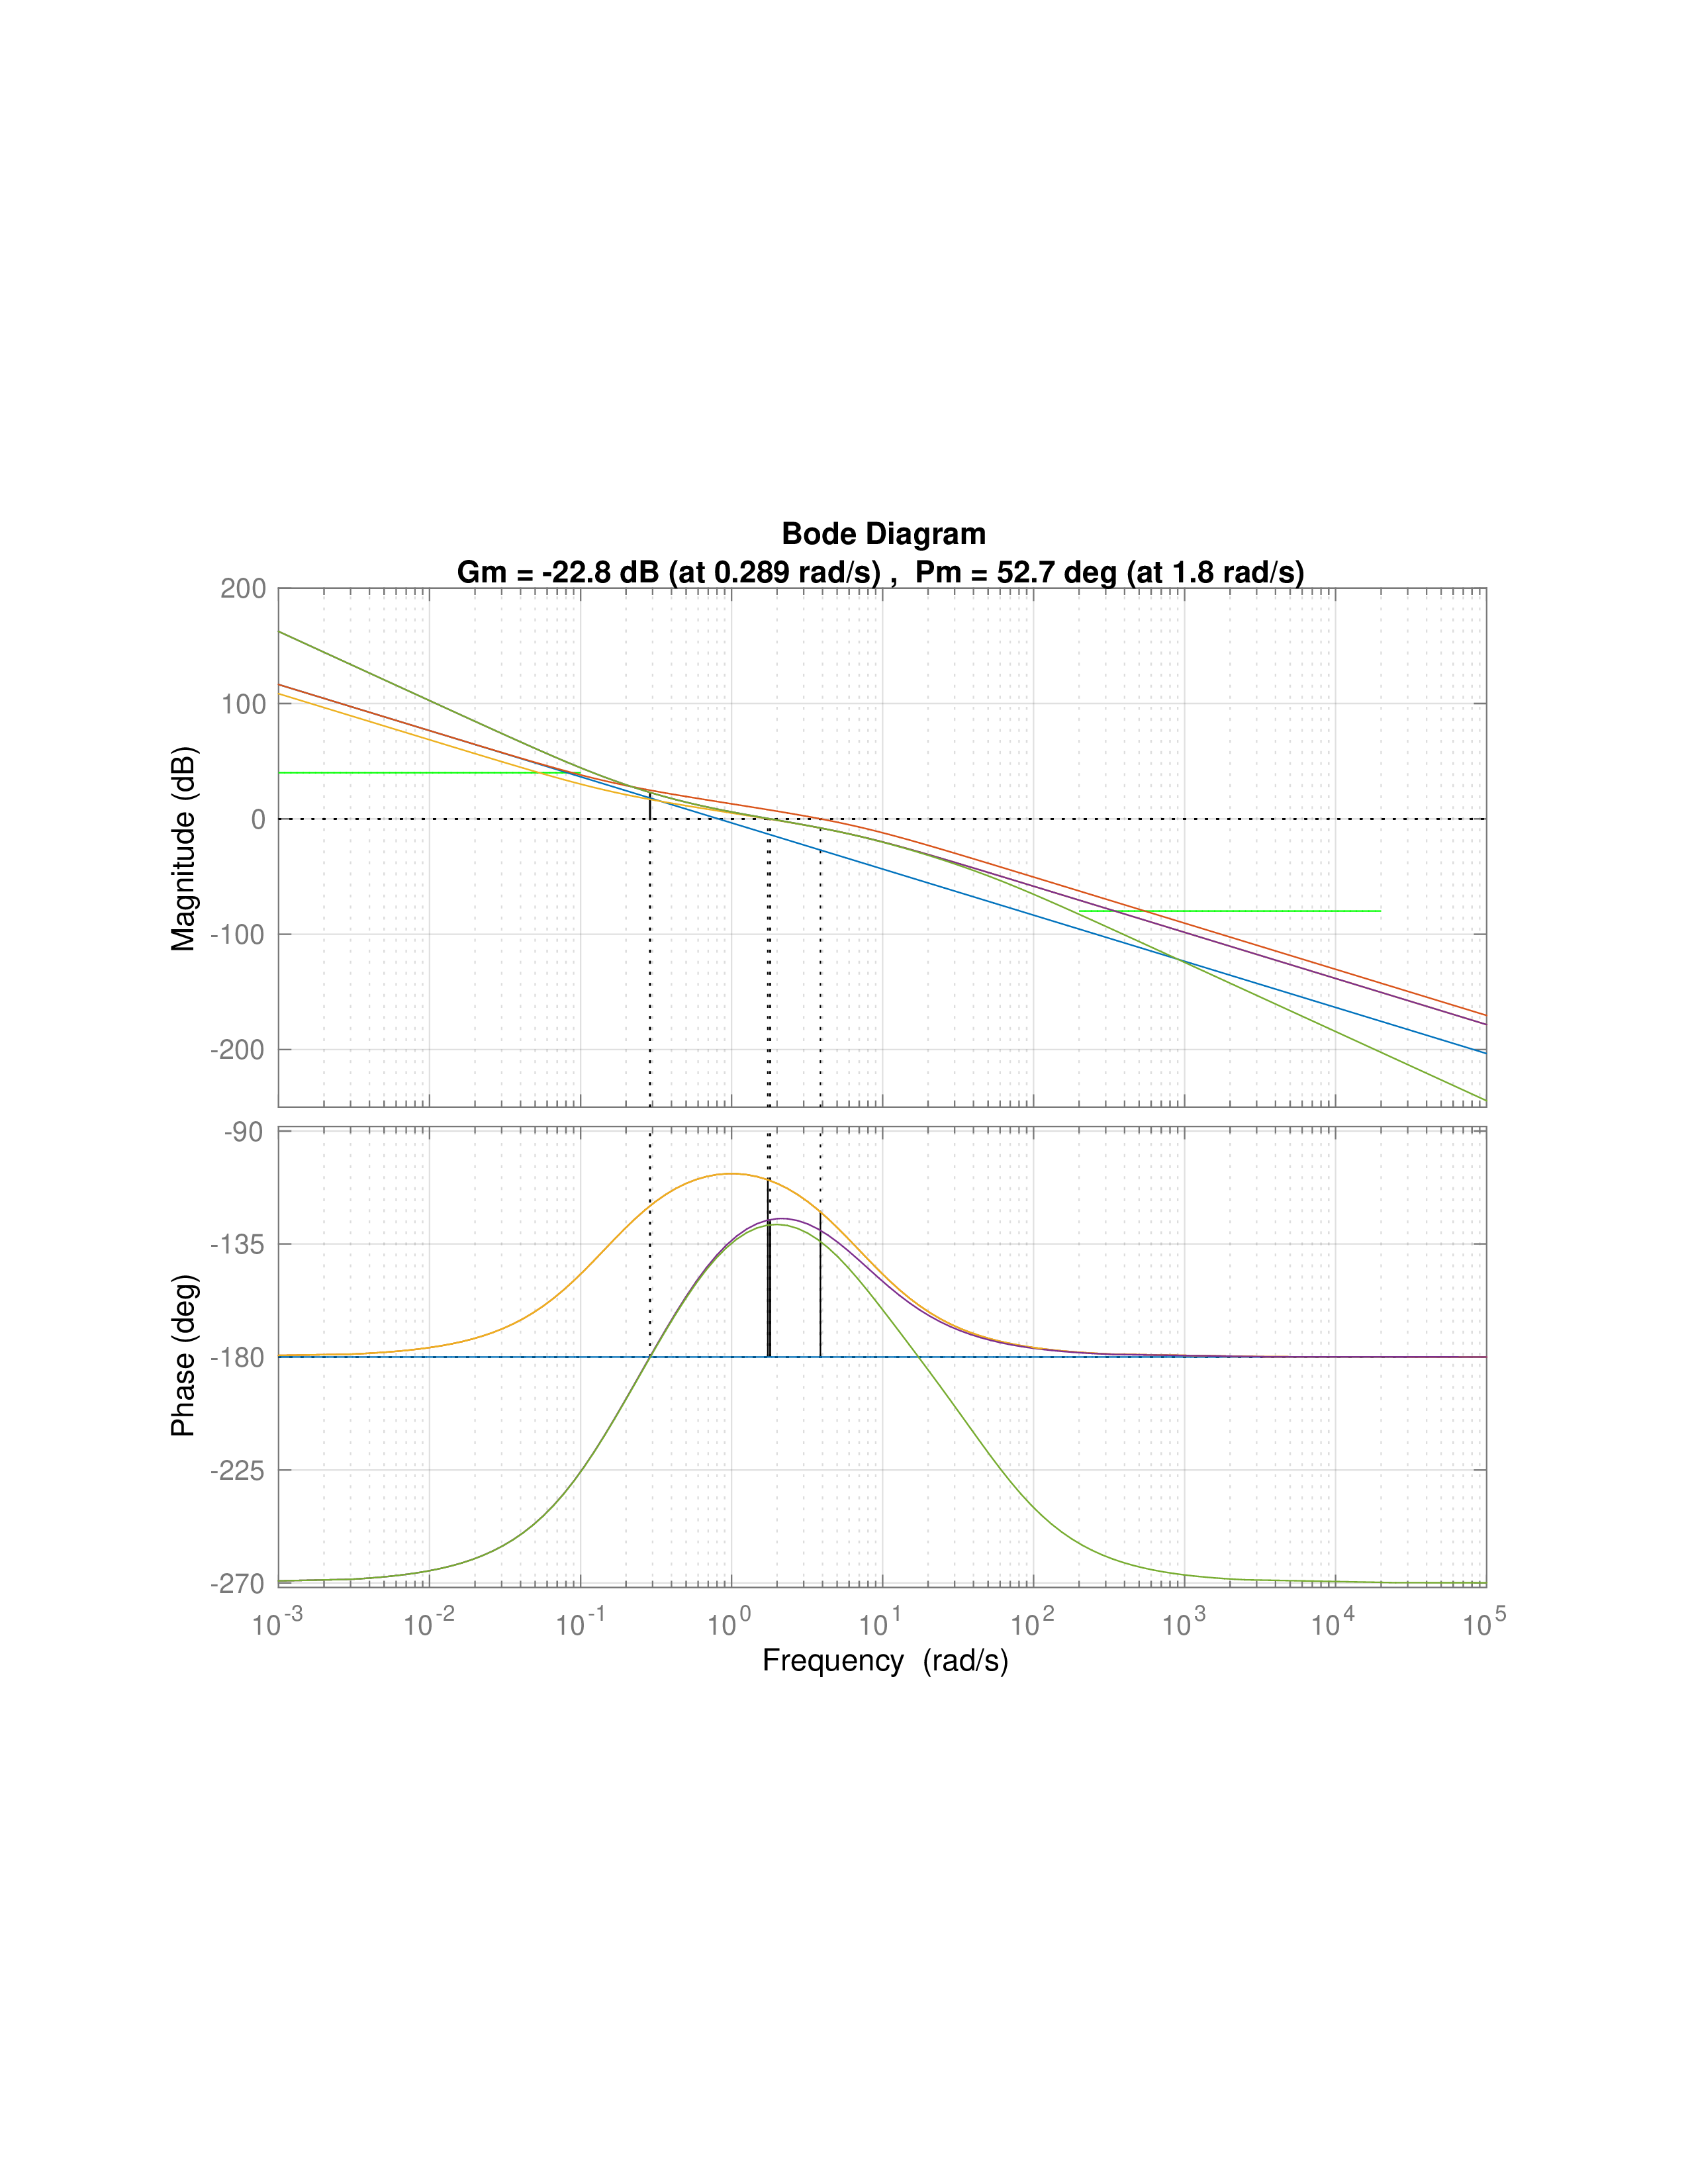
\includegraphics[width=0.95\textwidth]{6_design_studies/figures/hw_vtol_lon_compensator_design_4.pdf}
   \caption{The Bode plot for the system in HW~\ref{hw:vtol}.\ref{chap:loopshaping_design}, with phase lead, proportional, integral control, and a low pass  filter.}
   \label{fig:hw_vtol_lon_compensator_design_4}
\end{figure}

Since the phase margin is $PM=52.7$~degrees, we consider the phase margin specification to be satisfied.
The resulting compensator is
\[
C(s) = 0.4\left(\frac{45(s+1/\sqrt{45})}{s+1/\sqrt{45}}\right)\left(\frac{s+0.5}{s}\right)\left(\frac{50}{s+50}\right).
\]
The closed loop response, 
as well as the unit step response for the output and control signal are all show in Figure~\ref{fig:hw_vtol_lon_compensator_design_5}, where the prefilter
\[
F(s) = \frac{1}{s+1}
\]
has been added to reduce the peaking in the closed loop response.
\begin{figure}[H]
   \centering
   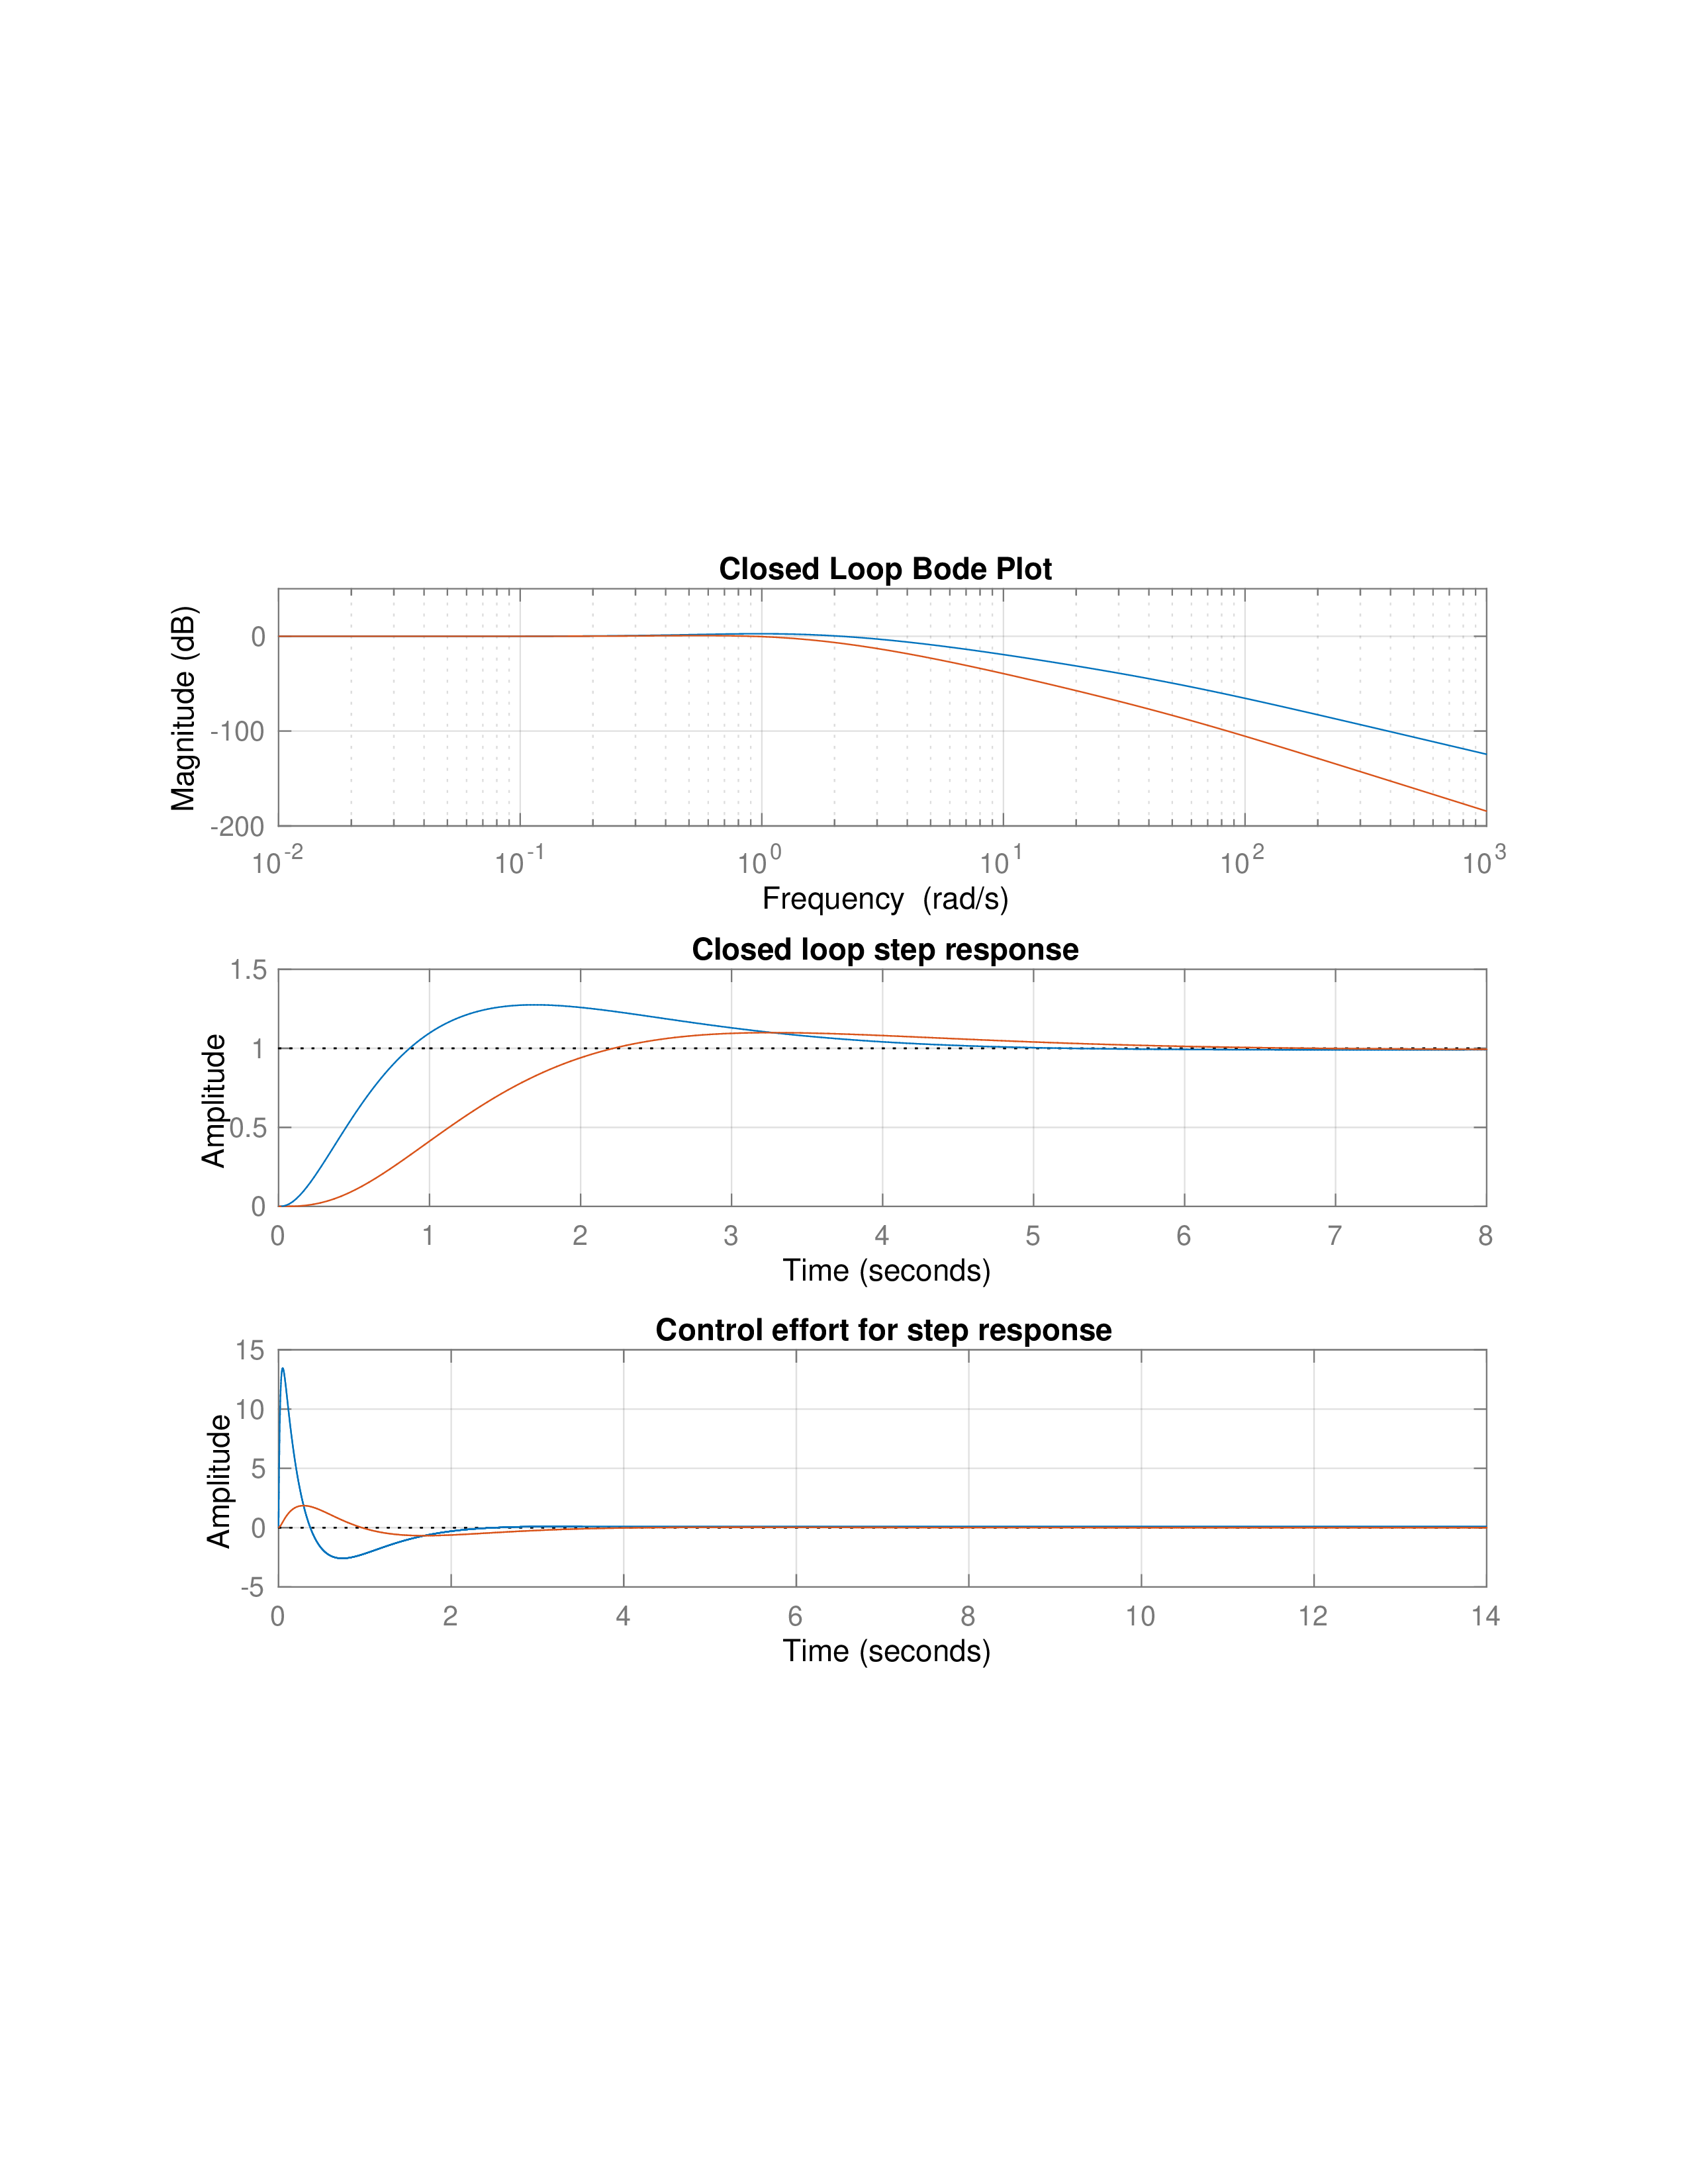
\includegraphics[width=0.95\textwidth]{6_design_studies/figures/hw_vtol_lon_compensator_design_5.pdf}
   \caption{The closed loop bode response, the unit step response for the output, and the unit step response for the input for the design in HW~\ref{hw:vtol}.\ref{chap:loopshaping_design}.}
   \label{fig:hw_vtol_lon_compensator_design_5}
\end{figure}

The Matlab code used to design the outer loop is shown below.
\begin{lstlisting}
Plant = P_lon;

%%%%%%%%%%%%%%%%%%%%%%%%%%%%%%%%%%%%%%%%%%%%%%%%%%%%%%%%%%%
%  Define Design Specifications
%%%%%%%%%%%%%%%%%%%%%%%%%%%%%%%%%%%%%%%%%%%%%%%%%%%%%%%%%%%

%--- general tracking specification ---
    omega_r = 10^(-1);  % track signals below this frequency
    gamma_r = 10^(-40/20);  % tracking error below this value
    w = logspace(log10(omega_r)-2,log10(omega_r));
        
%--- noise specification ---
    omega_n = 2*10^2;  % attenuate noise above this frequency
    gamma_n = 10^(-80/20);   % attenuate noise by this amount
    w = logspace(log10(omega_n),2+log10(omega_n));

%%%%%%%%%%%%%%%%%%%%%%%%%%%%%%%%%%%%%%%%%%%%%%%%%%%%%%%%%%%
% Control Design
  C = tf(1,1);
%%%%%%%%%%%%%%%%%%%%%%%%%%%%%%%%%%%%%%%%%%%%%%%%%%%%%%%%%%%

% phase lead: increase PM (stability)
    wmax = 1.0; % location of maximum frequency bump
    M    = 45; % separation between zero and pole
    Lead =tf(M*[1,wmax/sqrt(M)],[1,wmax*sqrt(M)]);
    C = C*Lead;

% proportional control: change cross over frequency
     kp = 0.4;
     C = C*kp;

% integral control: 
     k_I = 0.5; % frequency at which integral action ends
     Integrator = tf([1,k_I],[1,0]);
     C = C*Integrator;
    
% low pass filter: decrease gain at high frequency (noise)
     p = 50;
     LPF = tf(p,[1,p]);
     C = C*LPF;

%%%%%%%%%%%%%%%%%%%%%%%%%%%%%%%%%%%%%%%%%%%%%%%%%%%%%%%%%%%
% Prefilter Design
  F = tf(1,1);
%%%%%%%%%%%%%%%%%%%%%%%%%%%%%%%%%%%%%%%%%%%%%%%%%%%%%%%%%%%

% low pass filter
    p = 1;  % frequency to start the LPF
    LPF = tf(p, [1,p]);
    F = F*LPF;


       
%%%%%%%%%%%%%%%%%%%%%%%%%%%%%%%%%%%%%%%%%%%%%%%%%%%%%%%%%%%
% Convert controller to state space equations
%%%%%%%%%%%%%%%%%%%%%%%%%%%%%%%%%%%%%%%%%%%%%%%%%%%%%%%%%%%
[num,den] = tfdata(C,'v');
[P.A_lon_C,P.B_lon_C,P.C_lon_C,P.D_lon_C]=tf2ss(num,den);

[num,den] = tfdata(F,'v');
[P.A_lon_F, P.B_lon_F, P.C_lon_F, P.D_lon_F] = tf2ss(num,den);

C_lon = C;
\end{lstlisting}

%--------------------------------------------------------
(b)
From HW~\ref{hw:vtol}.\ref{chap:transfer_function_models}, the transfer function model for the inner loop is
\[
\tilde{\Theta}(s) = \frac{\left(\frac{1}{a_2}\right)}{s^2}\tilde{\tau}(s) = P_{lat_{in}}(s)\tilde{\tau}(s).
\]
Figure~\ref{fig:hw_vtol_lat_in_compensator_design_1} shows the Bode plot for $P_{lat_{in}}$. 
\begin{figure}[H]
   \centering
   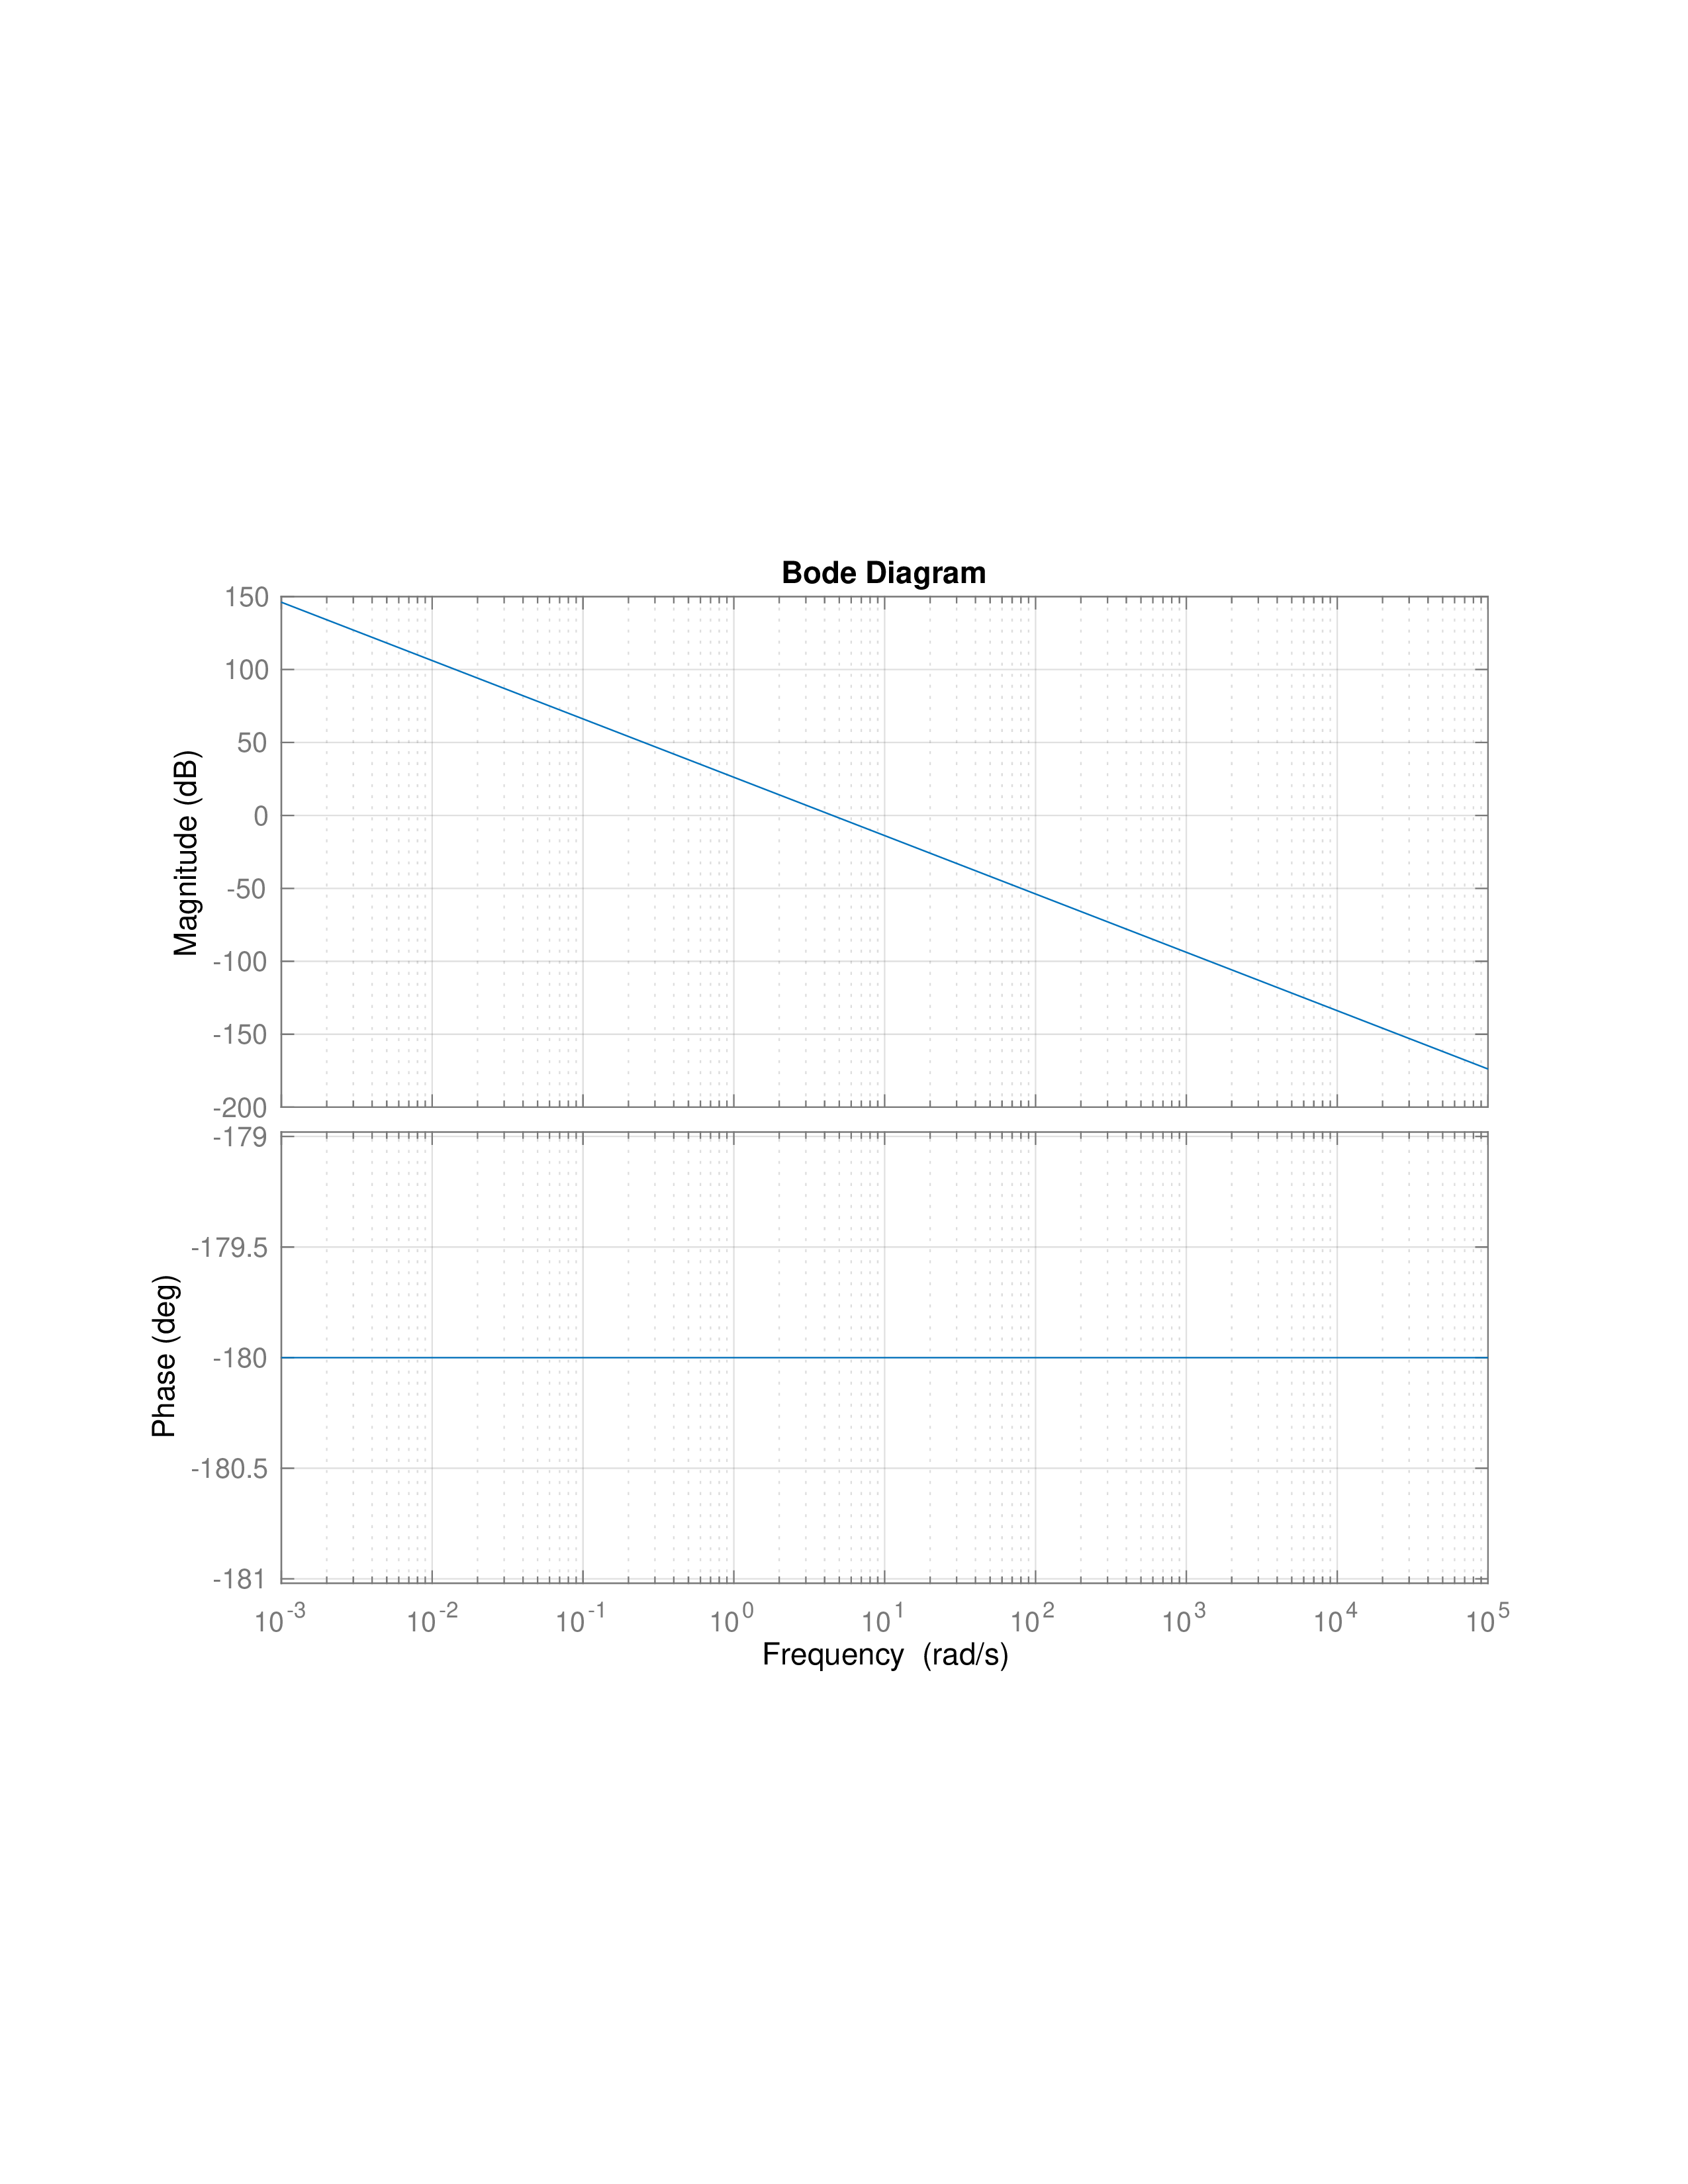
\includegraphics[width=0.95\textwidth]{6_design_studies/figures/hw_vtol_lat_in_compensator_design_1.pdf}
   \caption{The Bode plot for $P_{lat_{in}}$ in HW~\ref{hw:vtol}.\ref{chap:loopshaping_design}.}
   \label{fig:hw_vtol_lat_in_compensator_design_1}
\end{figure}

To stabilize the system, we add a phase lead element around the cross-over frequency.  Figure~\ref{fig:hw_vtol_lat_in_compensator_design_2} shows the loopgain with the addition of the phase lead filter
\[
C_{lead} = \frac{15(s+8/\sqrt{15})}{s+8/\sqrt{15}}.
\]
\begin{figure}[H]
   \centering
   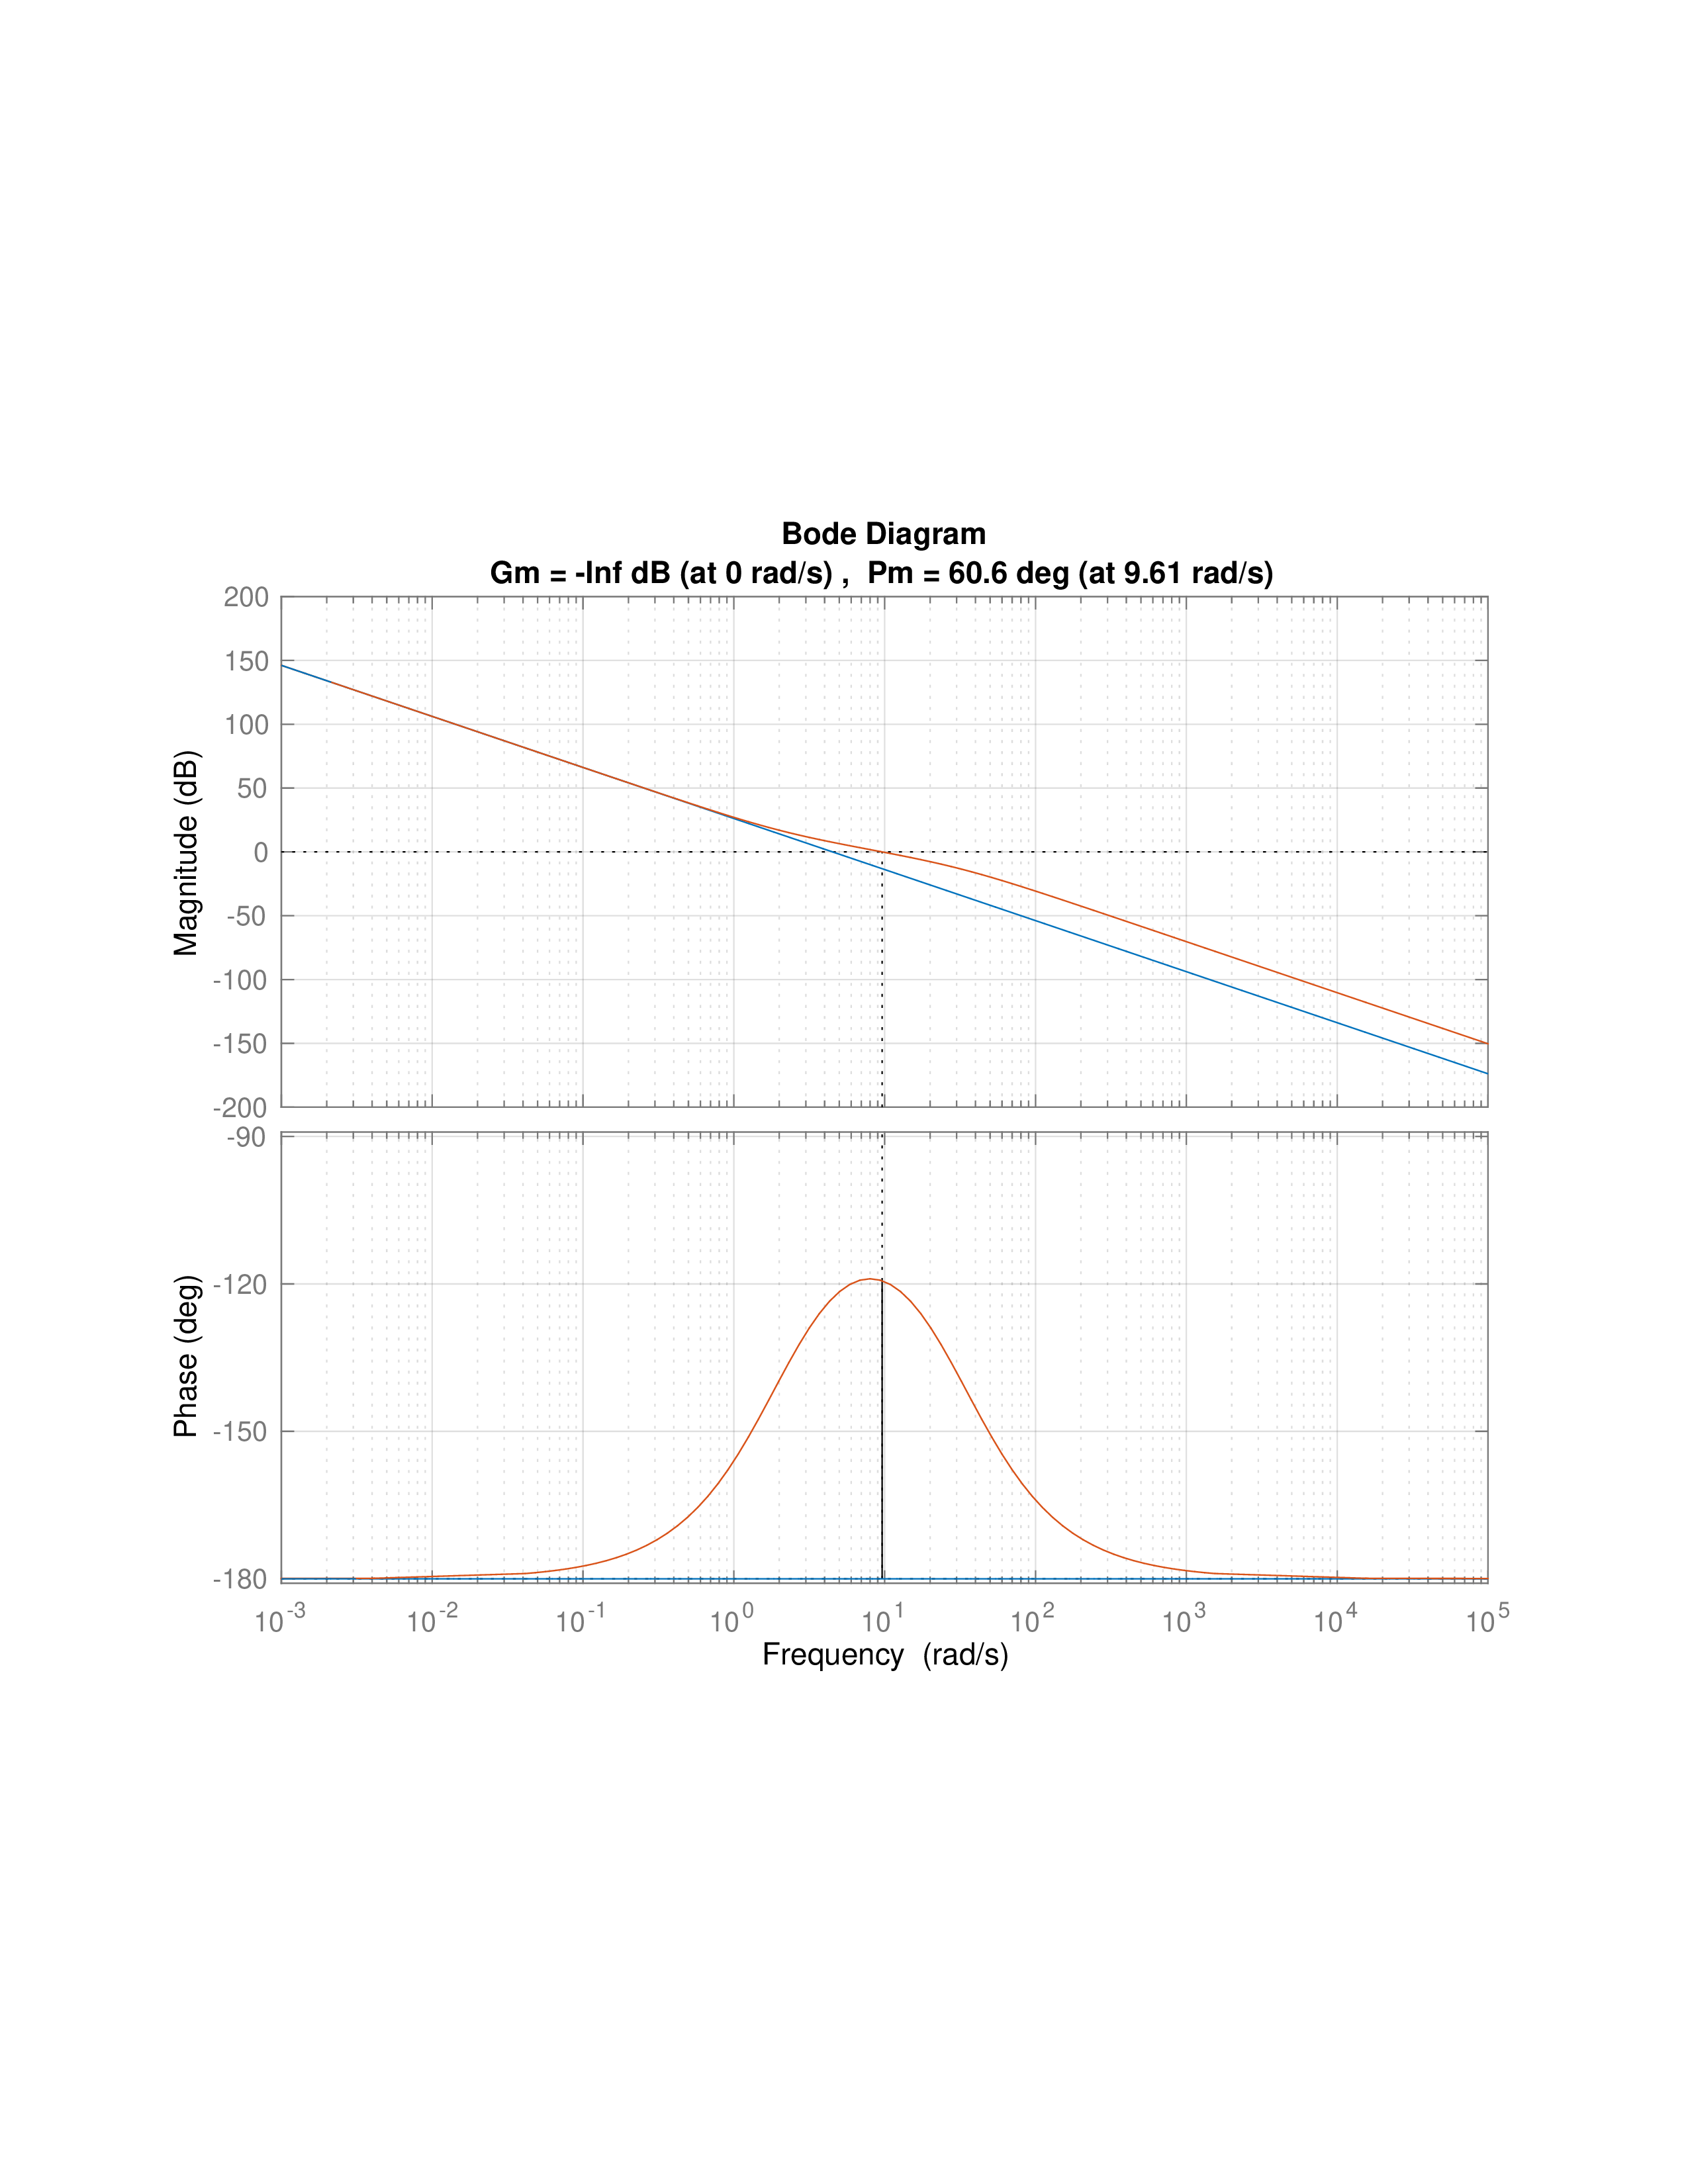
\includegraphics[width=0.95\textwidth]{6_design_studies/figures/hw_vtol_lat_in_compensator_design_2.pdf}
   \caption{The Bode plot for the inner loop of the lateral system in HW~\ref{hw:vtol}.\ref{chap:loopshaping_design}, with phase lead control.}
   \label{fig:hw_vtol_lat_in_compensator_design_2}
\end{figure}
Since the bandwidth and phase margin specifications are satisfied, we complete the design by adding the low pass filter
\[
C_{lpf} = \frac{200}{s+200}
\]
and the result is shown in Figure~\ref{fig:hw_vtol_lat_in_compensator_design_3}.
\begin{figure}[H]
   \centering
   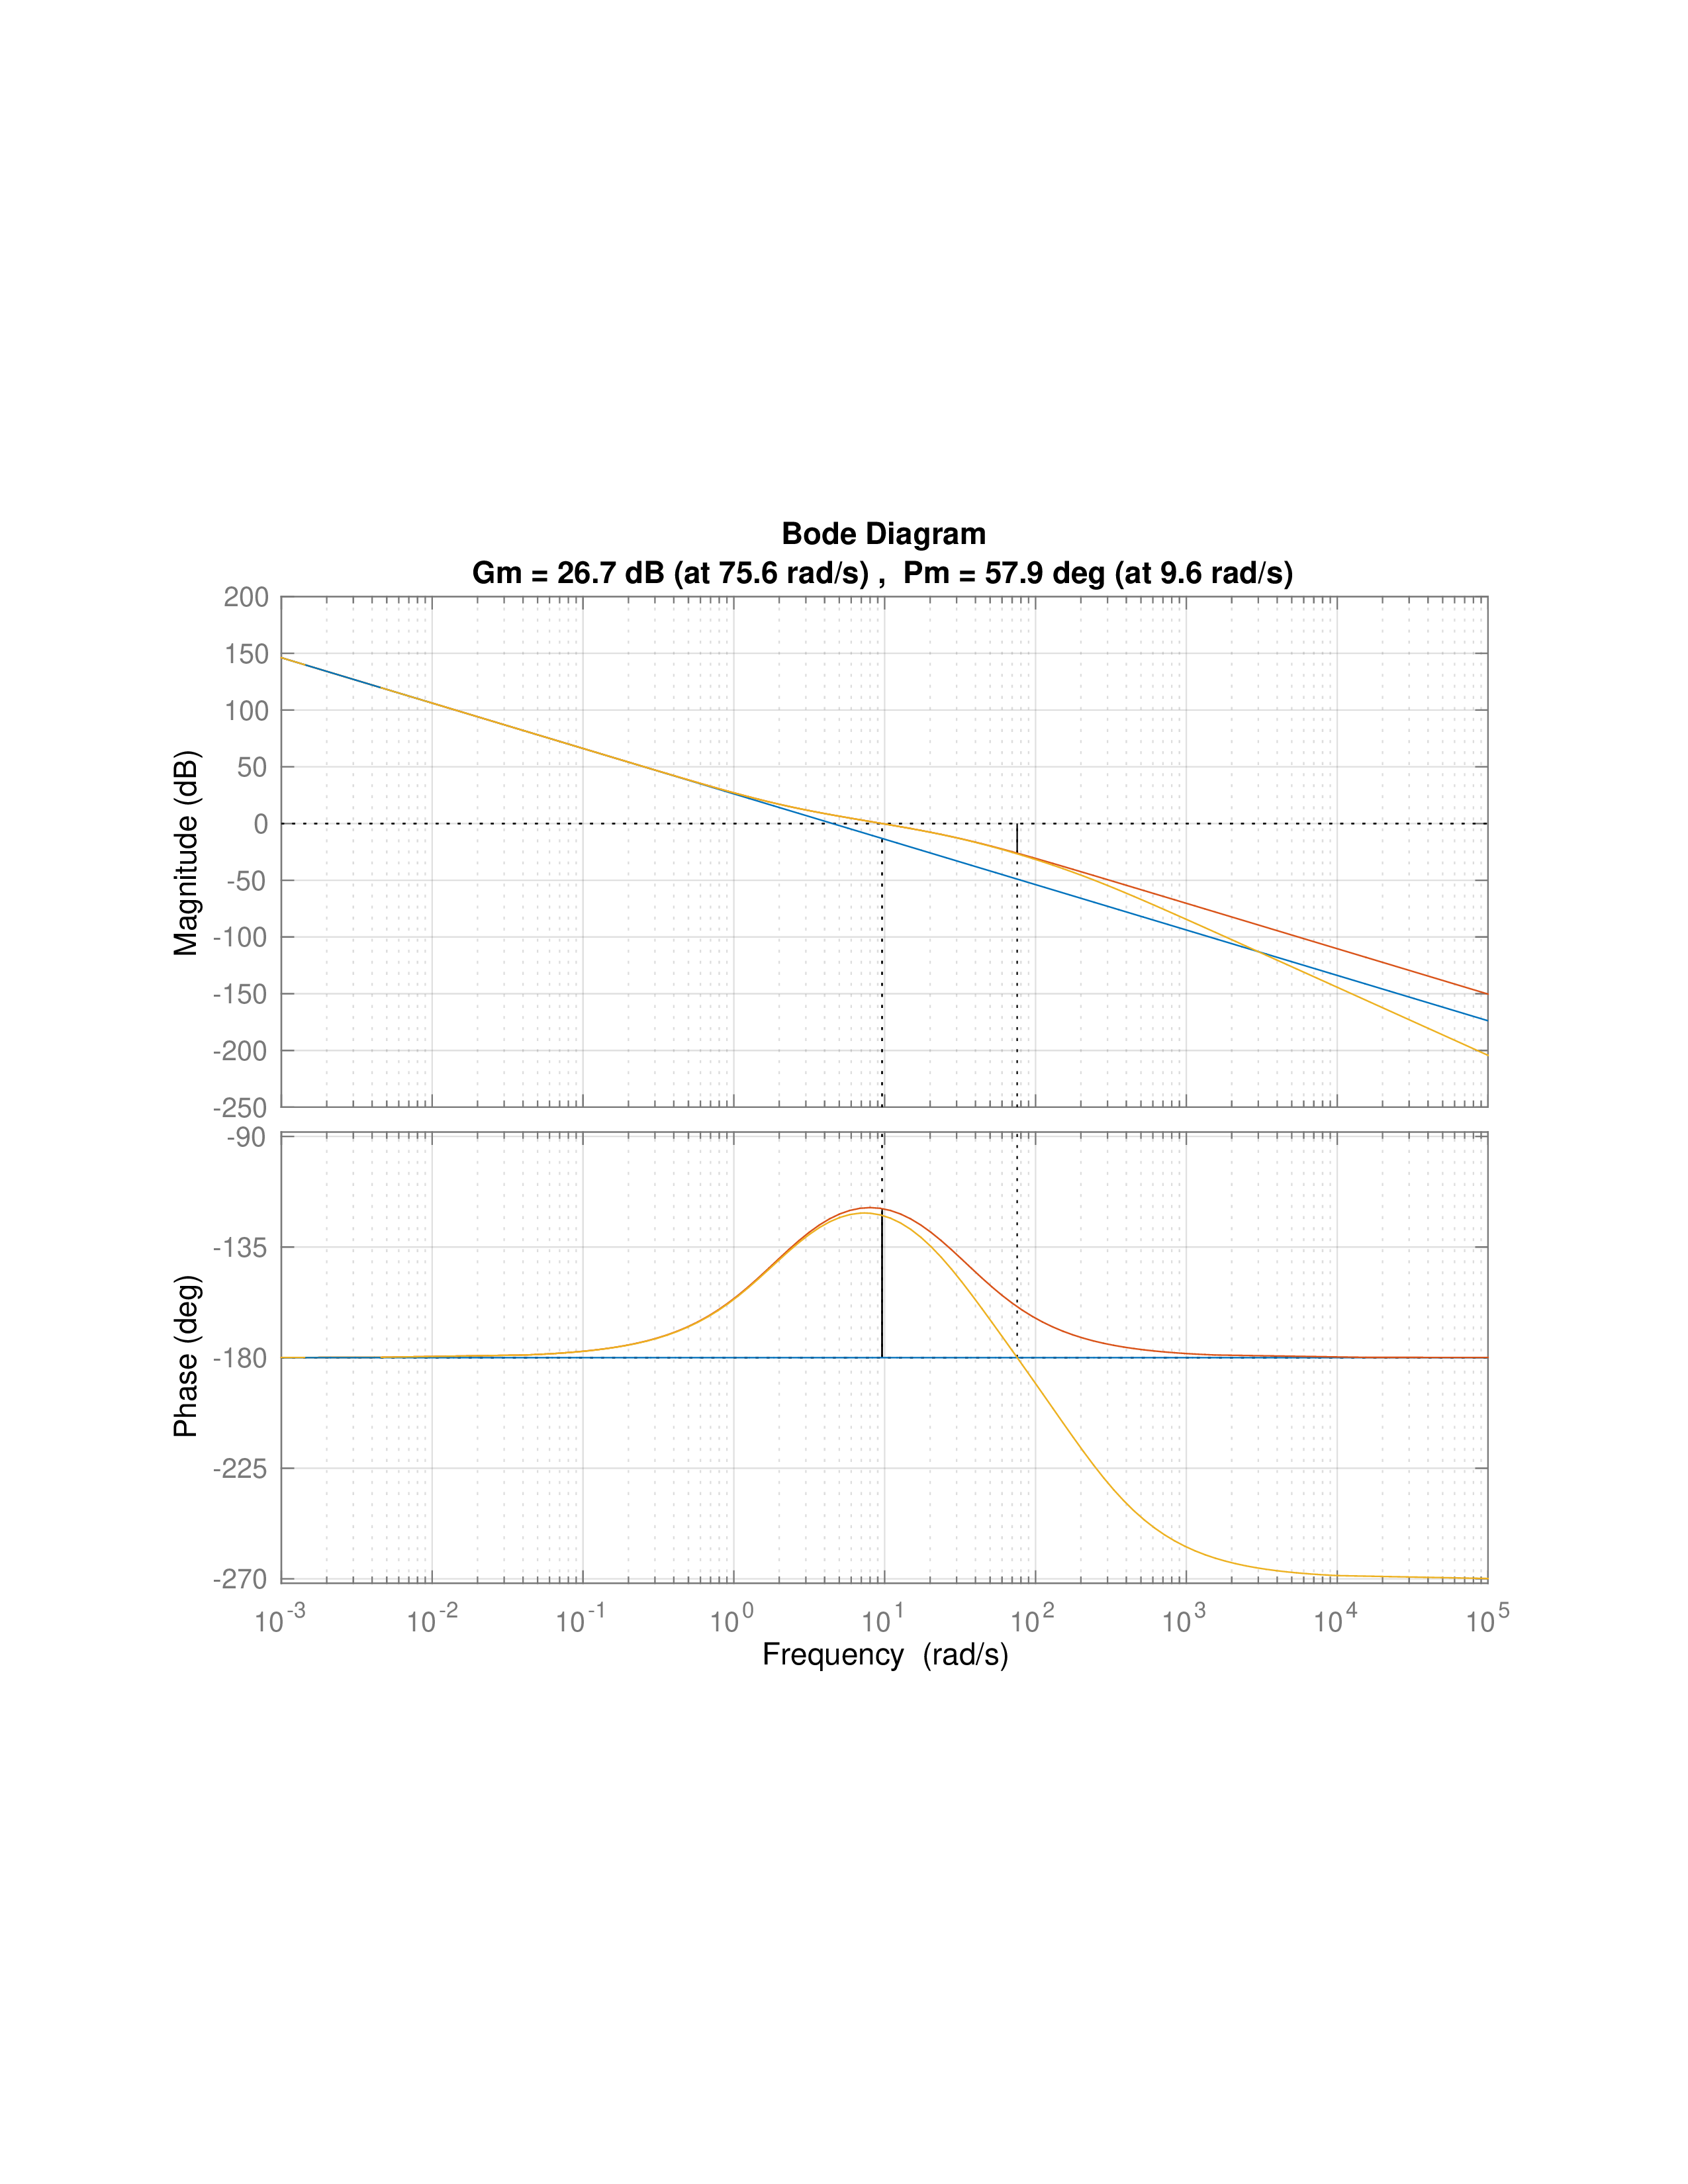
\includegraphics[width=0.95\textwidth]{6_design_studies/figures/hw_vtol_lat_in_compensator_design_3.pdf}
   \caption{The Bode plot for the inner loop of the lateral system in HW~\ref{hw:vtol}.\ref{chap:loopshaping_design}, with phase lead control, and a low pass  filter.}
   \label{fig:hw_vtol_lat_in_compensator_design_3}
\end{figure}
The resulting compensator is
\[
C(s) = \left(\frac{15(s+8/\sqrt{15})}{s+8\sqrt{15}}\right)\left(\frac{200}{s+200}\right).
\]
The closed loop response, 
as well as the unit step response for the output and control signal are all show in Figure~\ref{fig:hw_vtol_lat_in_compensator_design_4}.
\begin{figure}[H]
   \centering
   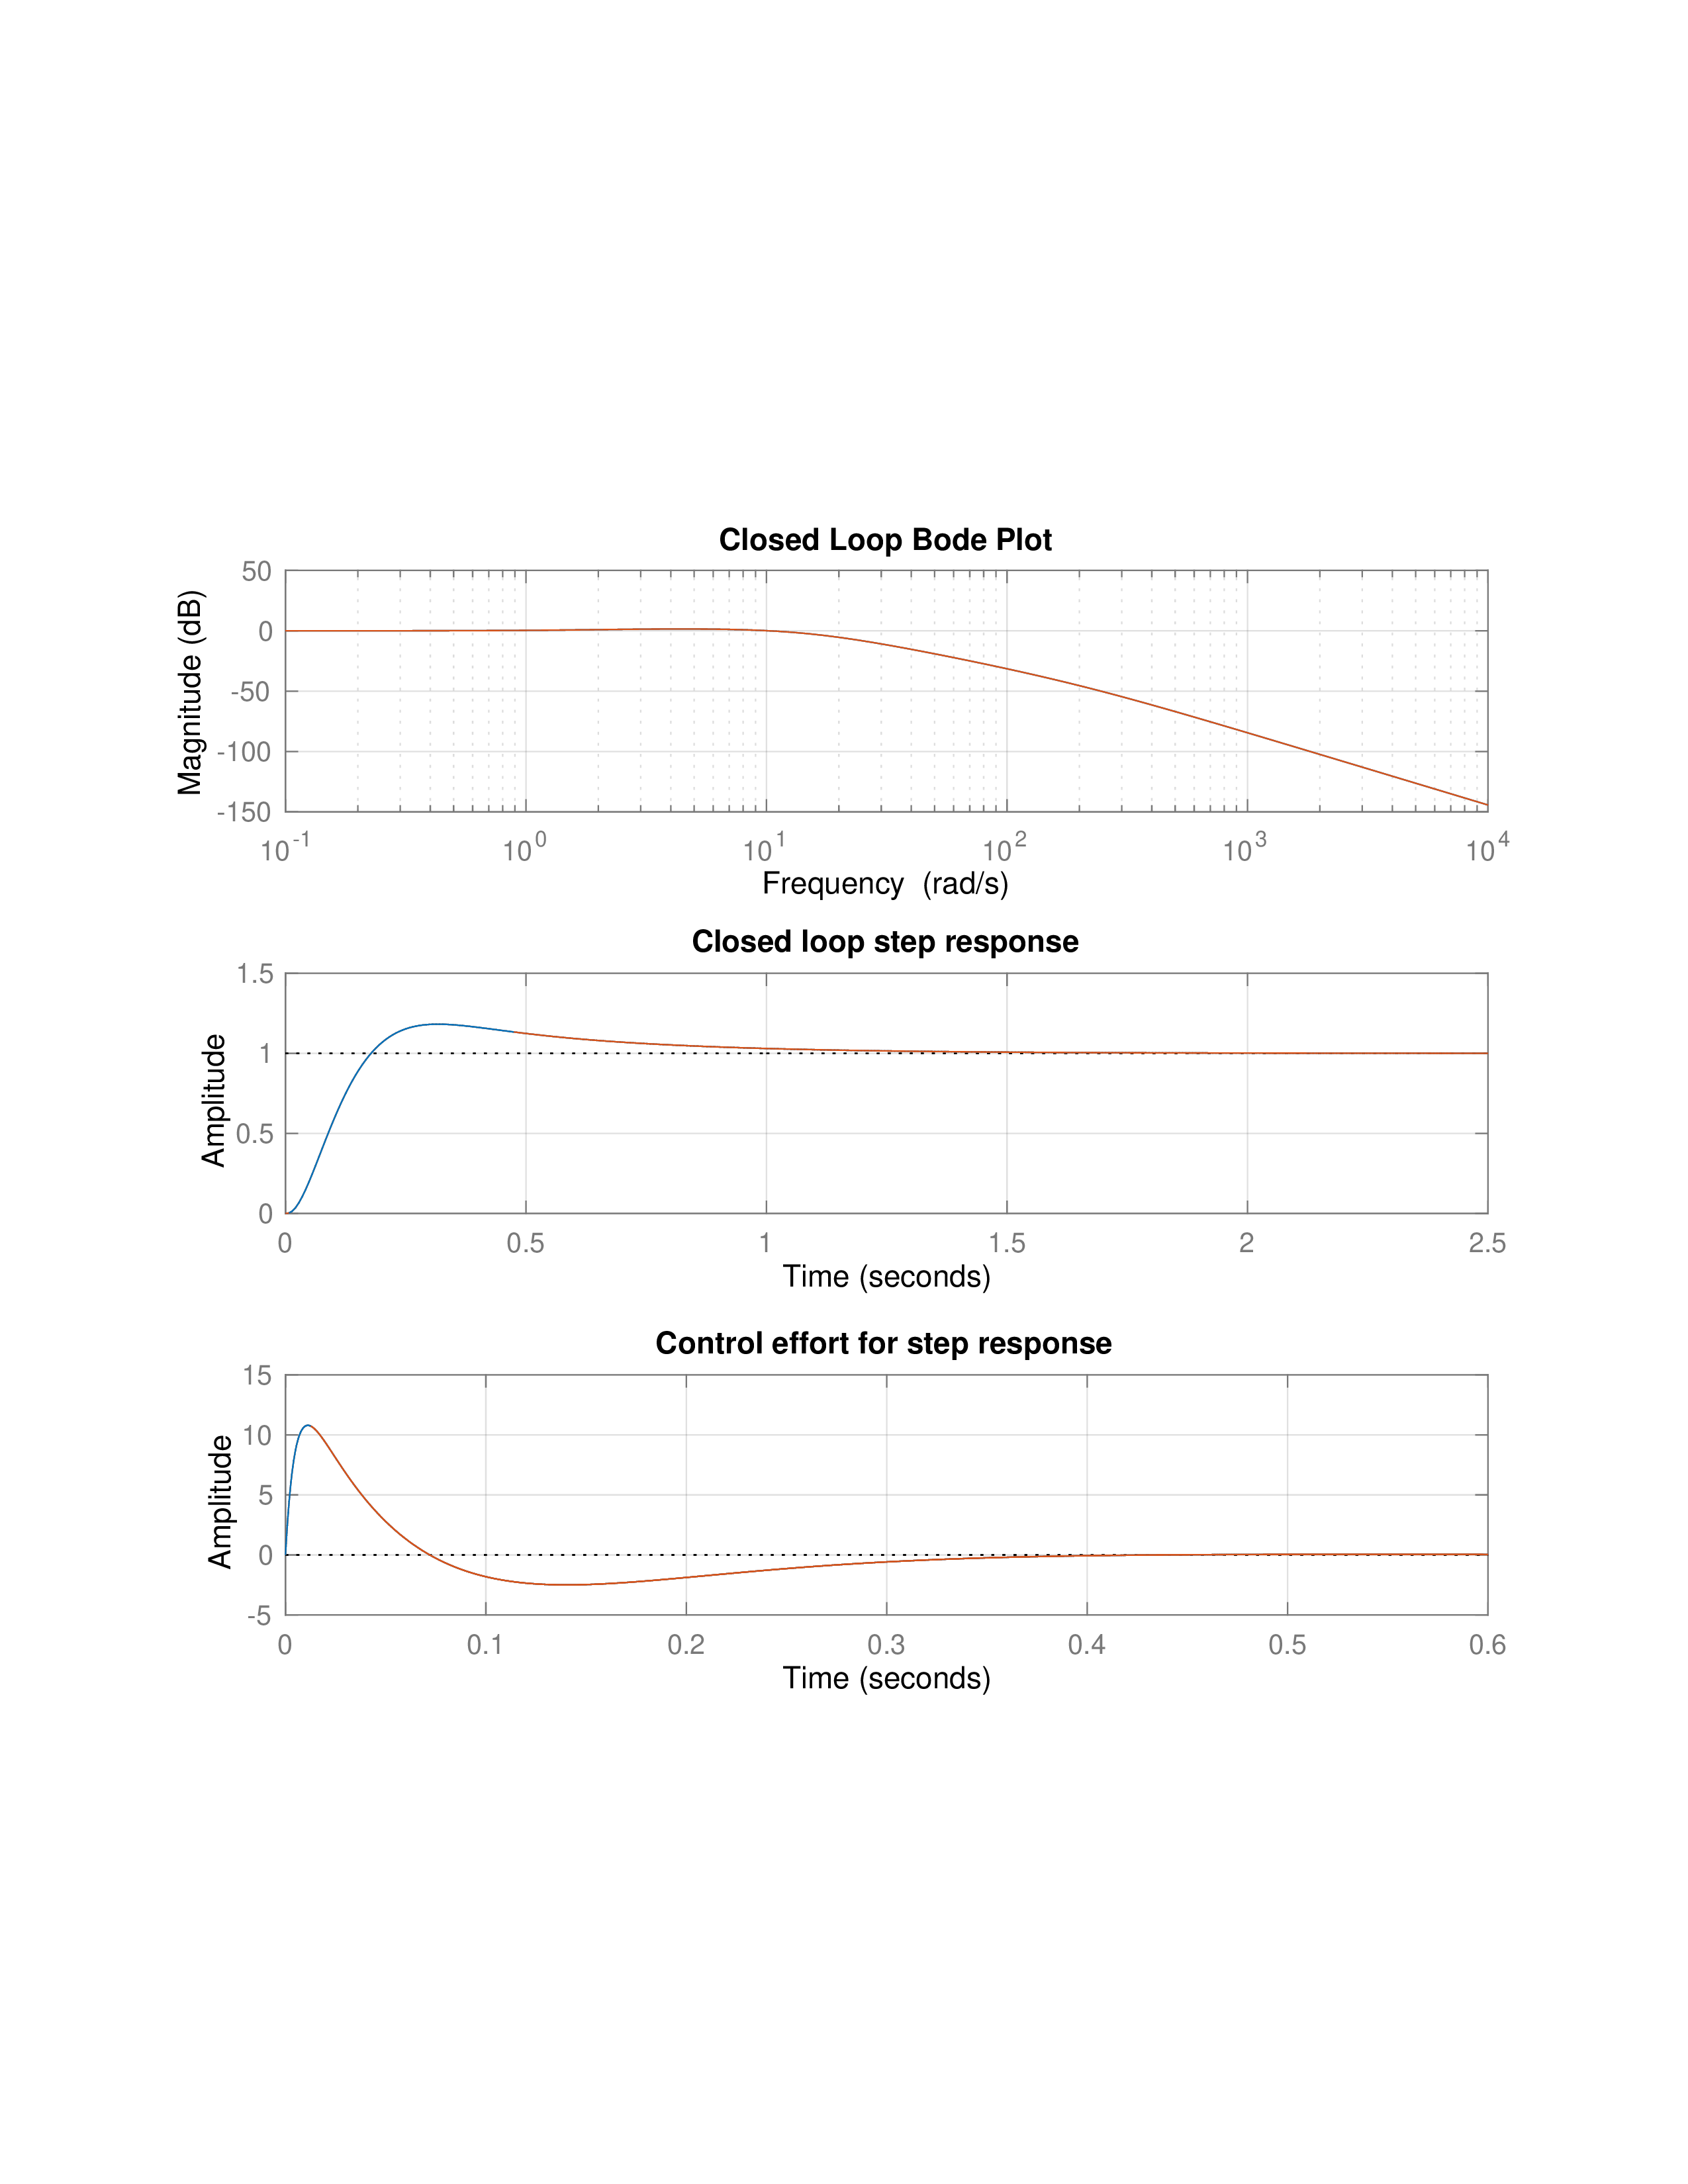
\includegraphics[width=0.95\textwidth]{6_design_studies/figures/hw_vtol_lat_in_compensator_design_4.pdf}
   \caption{The closed loop bode response, the unit step response for the output, and the unit step response for the input for the inner loop lateral design in HW~\ref{hw:vtol}.\ref{chap:loopshaping_design}.}
   \label{fig:hw_vtol_lat_in_compensator_design_4}
\end{figure}

The Matlab code used to design the outer loop is shown below.
\begin{lstlisting}
Plant = P_lat_in;


%%%%%%%%%%%%%%%%%%%%%%%%%%%%%%%%%%%%%%%%%%%%%%%%%%%%%%%%%%%
% Control Design
  C = tf(1,1);
%%%%%%%%%%%%%%%%%%%%%%%%%%%%%%%%%%%%%%%%%%%%%%%%%%%%%%%%%%%

% phase lead: increase PM (stability)
    wmax = 8.0; % location of maximum frequency bump
    M    = 15; % separation between zero and pole
    Lead =tf(M*[1,wmax/sqrt(M)],[1,wmax*sqrt(M)]);
    C = C*Lead;
    
% low pass filter: decrease gain at high frequency (noise)
     p = 200;
     LPF = tf(p,[1,p]);
     C = C*LPF;
%%%%%%%%%%%%%%%%%%%%%%%%%%%%%%%%%%%%%%%%%%%%%%%%%%%%%%%%%%%
% Convert controller to state space equations 
%%%%%%%%%%%%%%%%%%%%%%%%%%%%%%%%%%%%%%%%%%%%%%%%%%%%%%%%%%%
[num,den] = tfdata(C,'v');
[P.A_lat_in_C,P.B_lat_in_C,P.C_lat_in_C,P.D_lat_in_C]=...
    tf2ss(num,den);

C_lat_in = C;
\end{lstlisting}


%--------------------------------------------------------
(c)

From HW~\ref{hw:vtol}.\ref{chap:transfer_function_models}, the transfer function model is
\[
Z(s) = \frac{-\left(\frac{F_0}{a_1}\right)}{s^2 + \frac{\mu}{a_1}} \tilde{\Theta}(s) = P_{lat_{out}}(s)\tilde{\Theta}(s).
\]
Figure~\ref{fig:hw_vtol_lat_out_compensator_design_1} shows the Bode plot for $P_{lat_{out}}$ together with the design specification on attenuating the noise.  The requirement to reject constant input disturbances requires the inclusion of an integrator which is not shown in Figure~\ref{fig:hw_vtol_lat_out_compensator_design_1}.
%
\begin{figure}[H]
   \centering
   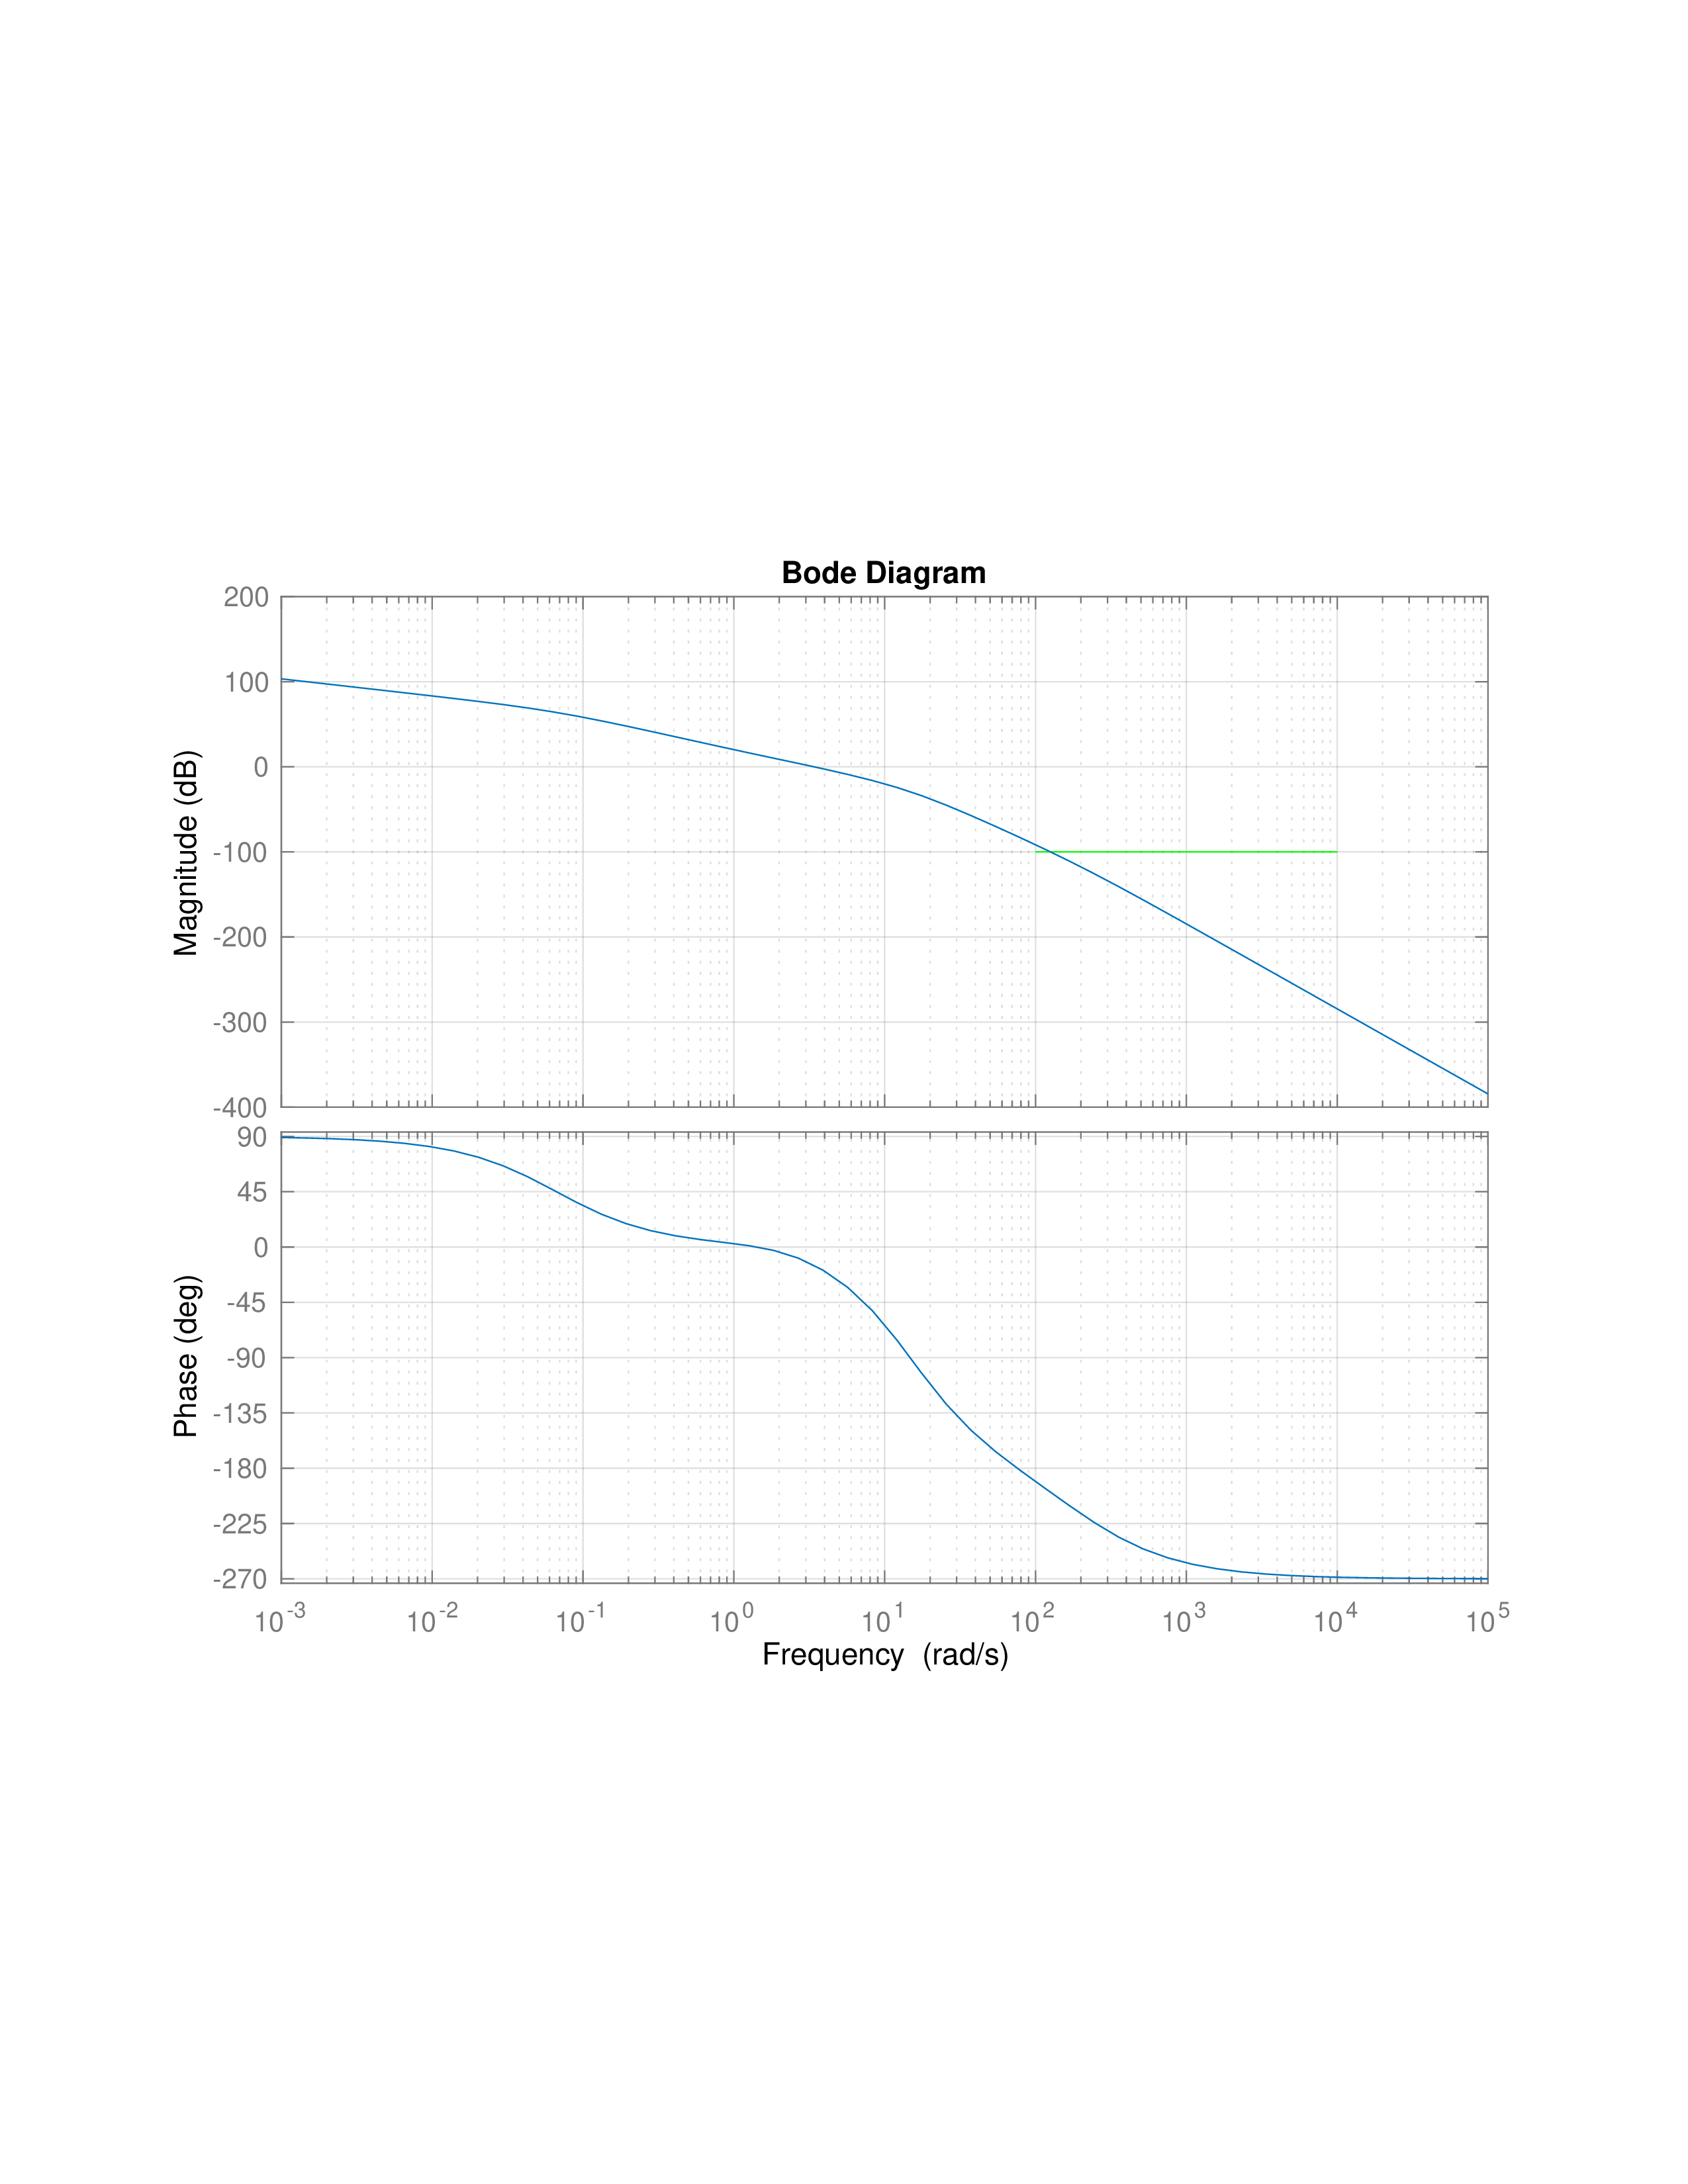
\includegraphics[width=0.95\textwidth]{6_design_studies/figures/hw_vtol_lat_out_compensator_design_1.pdf}
   \caption{The Bode plot for the outer loop of the lateral system in HW~\ref{hw:vtol}.\ref{chap:loopshaping_design}, together with the design specifications.}
   \label{fig:hw_vtol_lat_out_compensator_design_1}
\end{figure}

Since the gain of the open loop plant is negative, a negative proportional gain is needed to stabilize the system.  To place the cross over frequency at the correct location, a proportional gain of $k_P = -0.03$ is selected.  The resulting loop gain is shown in Figure~\ref{fig:hw_vtol_lat_out_compensator_design_2}
\begin{figure}[H]
   \centering
   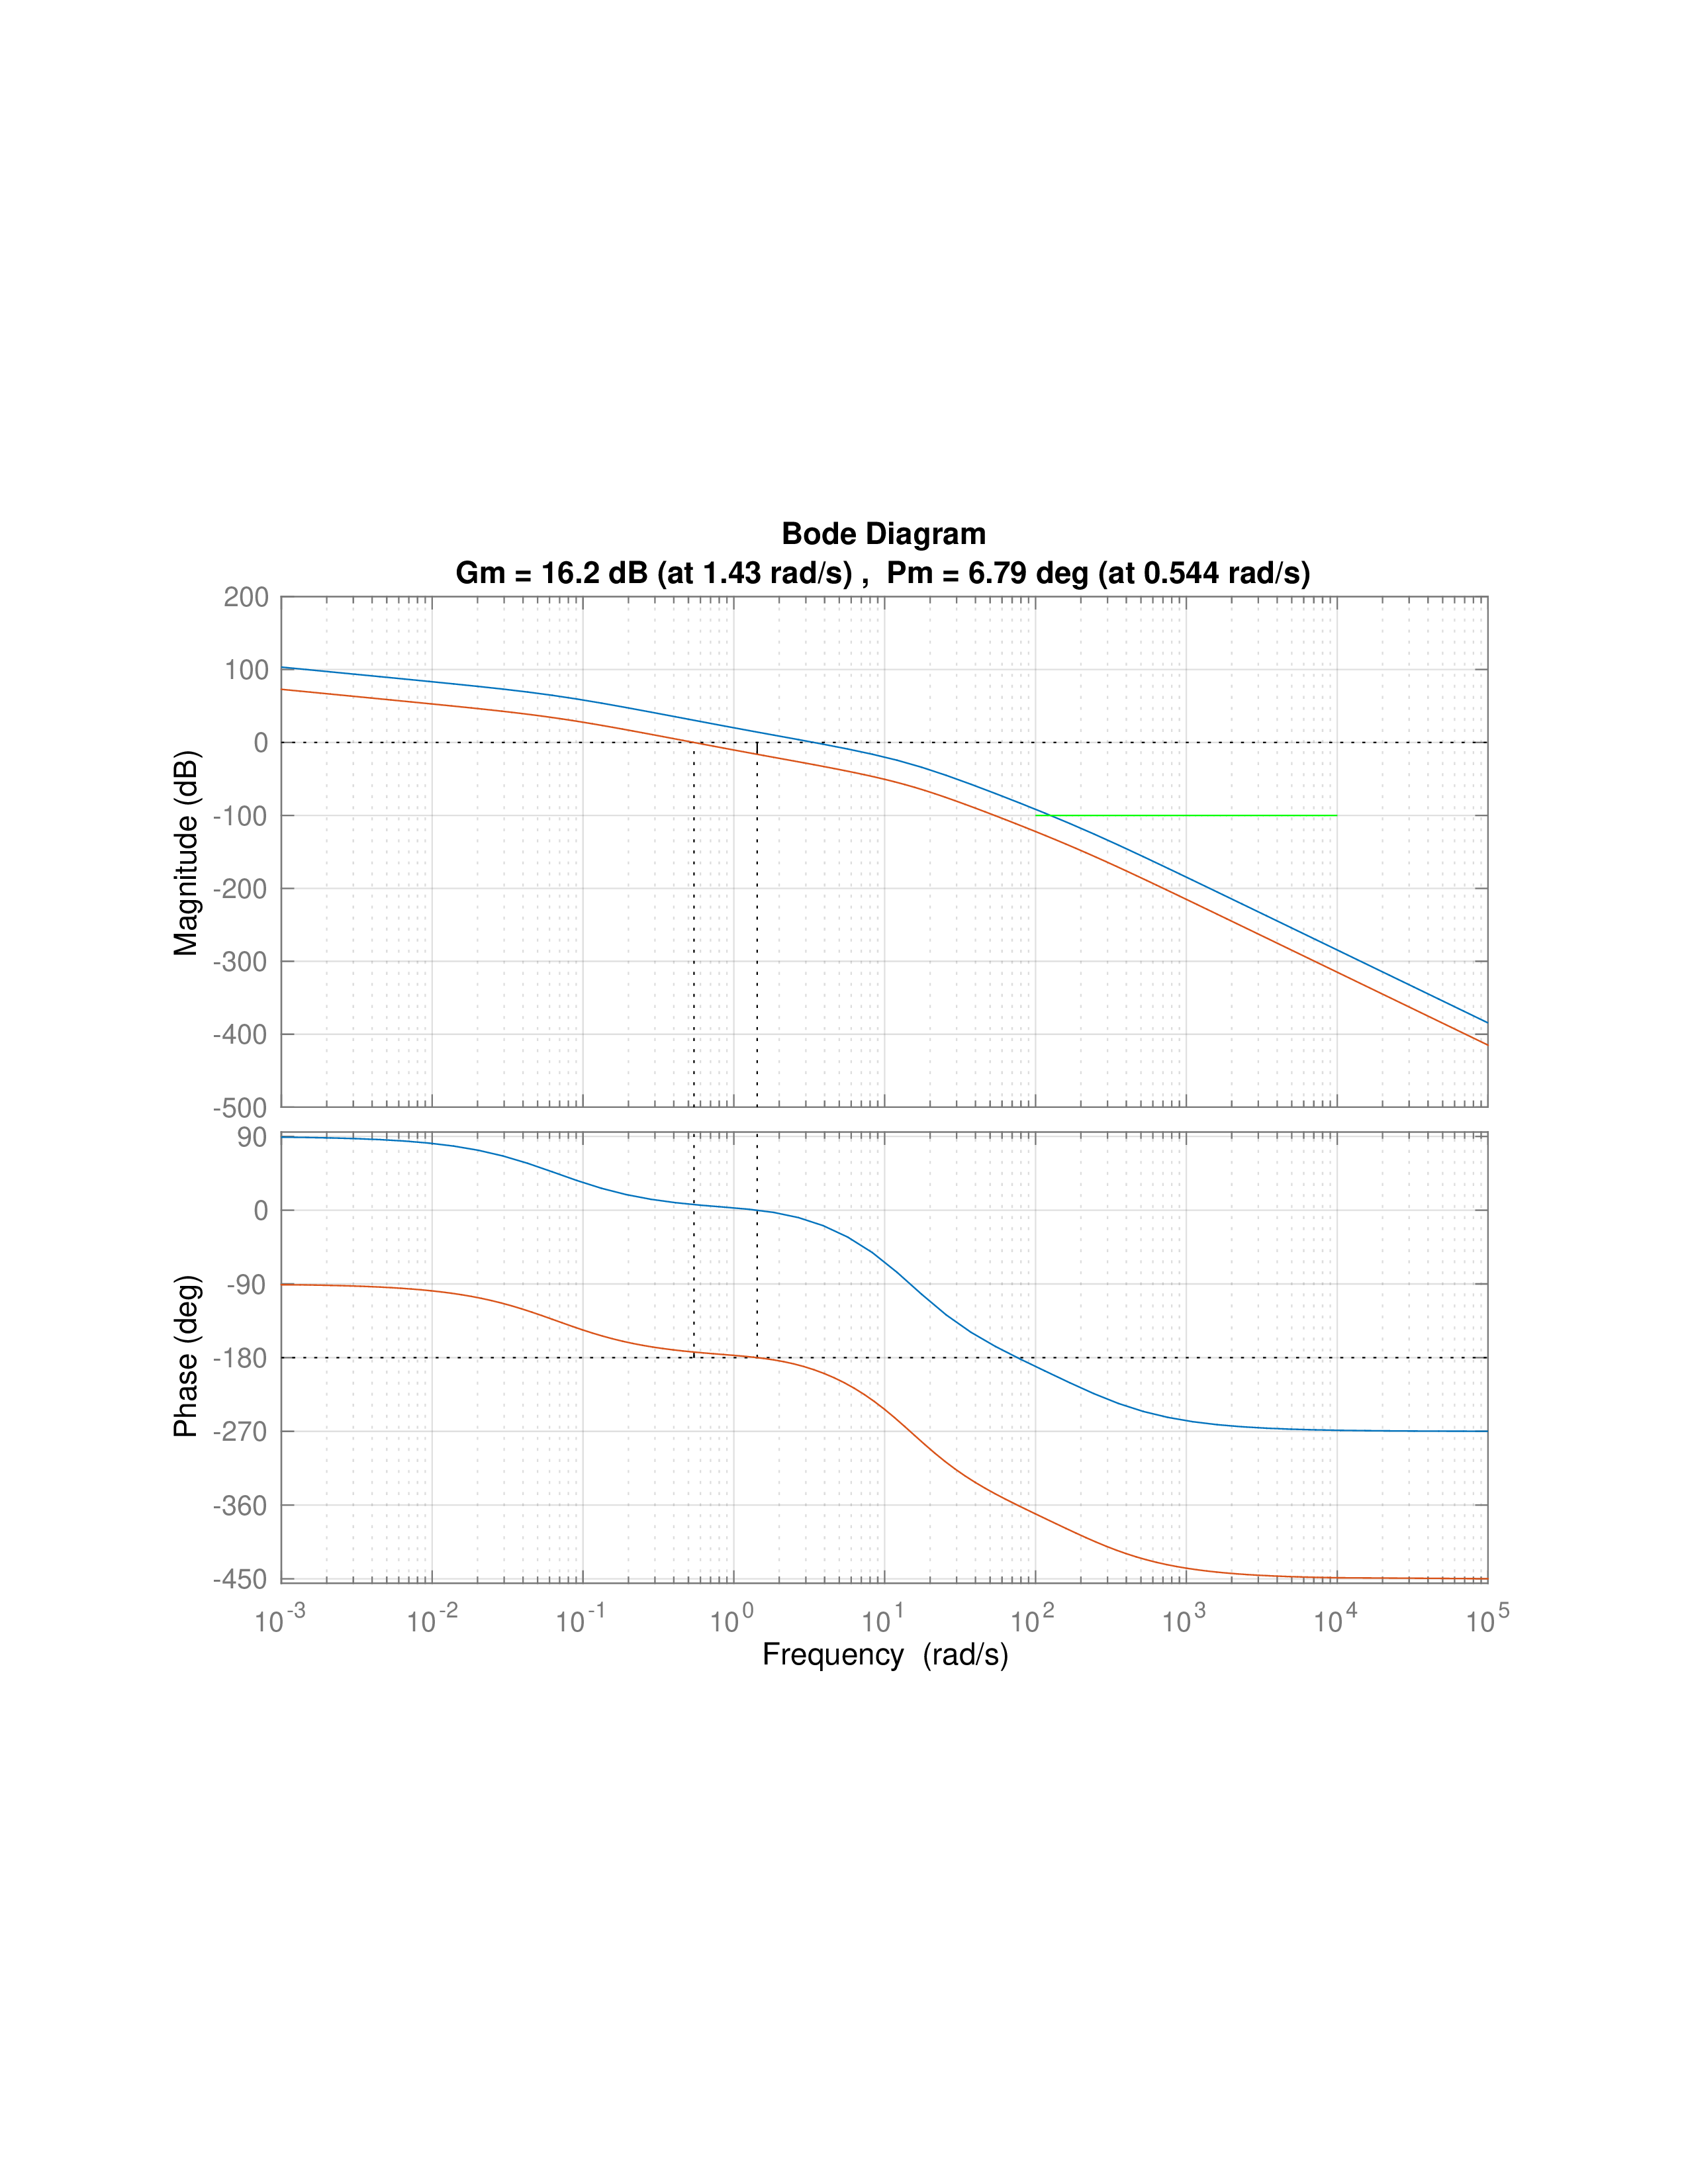
\includegraphics[width=0.95\textwidth]{6_design_studies/figures/hw_vtol_lat_out_compensator_design_2.pdf}
   \caption{The Bode plot for the outer loop of the lateral system in HW~\ref{hw:vtol}.\ref{chap:loopshaping_design} with proportional gain $k_P=-0.03$.}
   \label{fig:hw_vtol_lat_out_compensator_design_2}
\end{figure}
To increase the phase margin, the phase lead element
\[
C_{lead} = \frac{45(s+1.3/\sqrt{45})}{s+1.3\sqrt{45}},
\]
is added, and the resulting loop gain is shown in Figure~\ref{fig:hw_vtol_lat_out_compensator_design_3}
\begin{figure}[H]
   \centering
   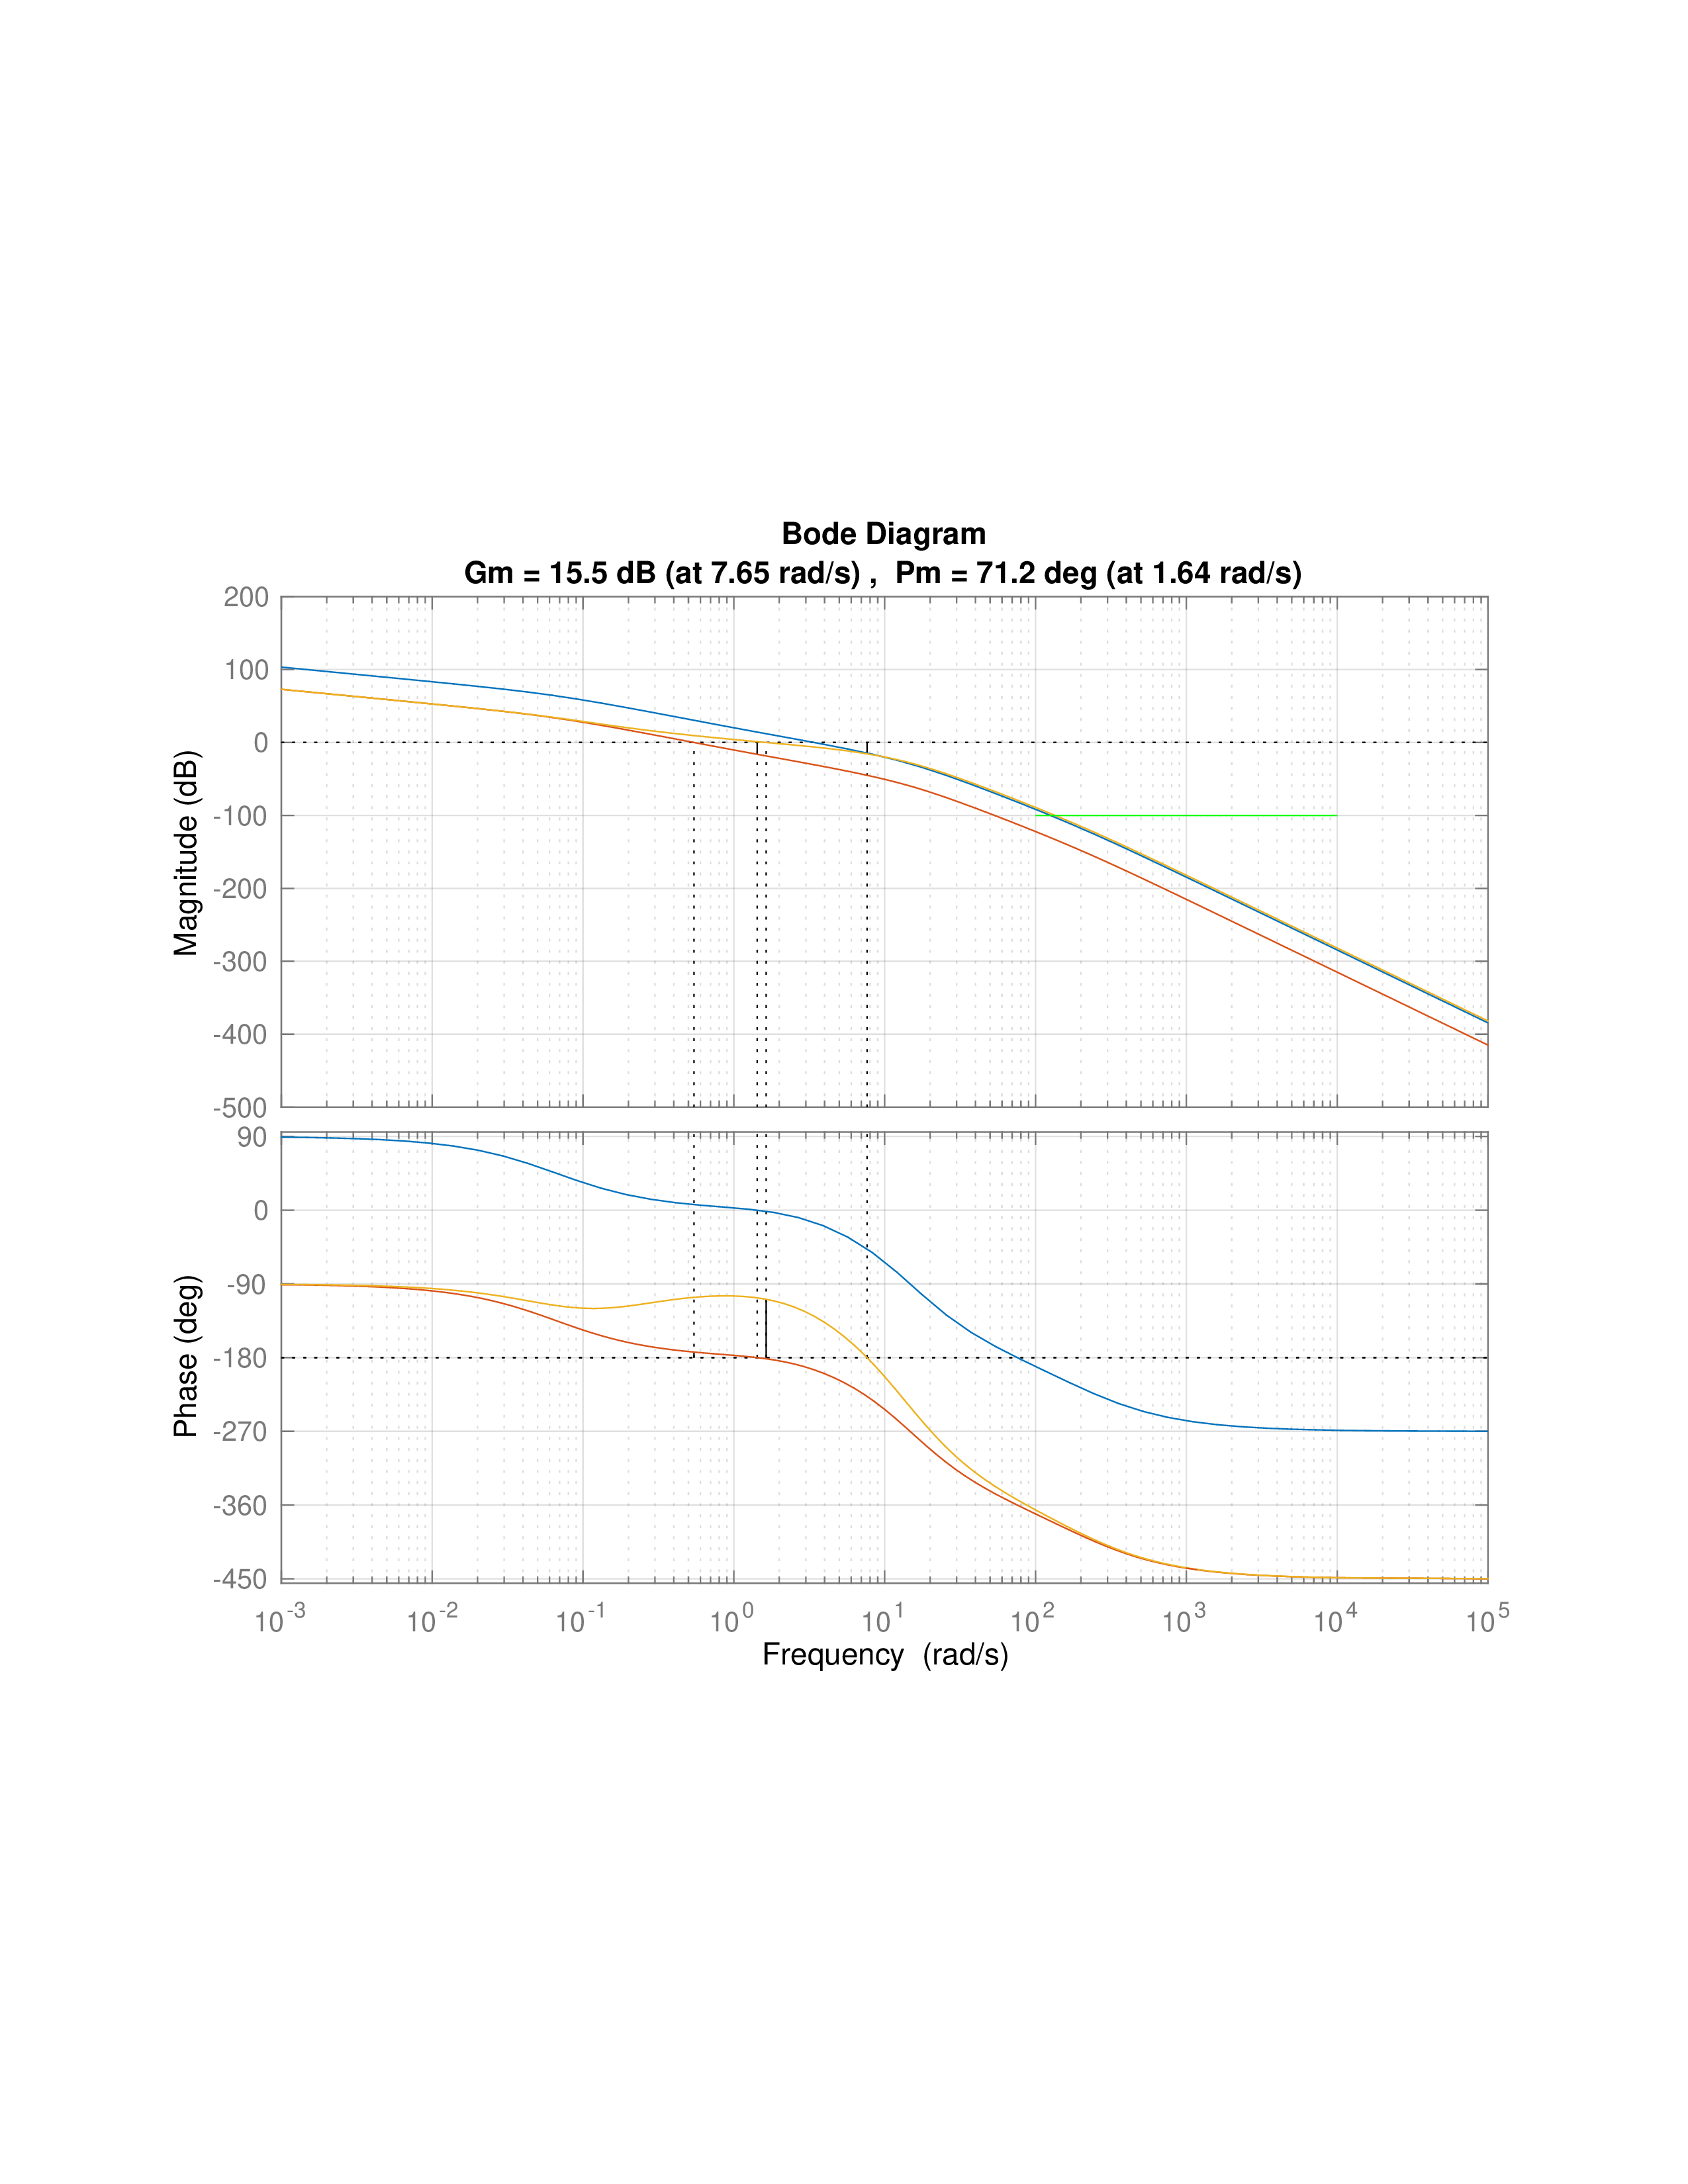
\includegraphics[width=0.95\textwidth]{6_design_studies/figures/hw_vtol_lat_out_compensator_design_3.pdf}
   \caption{The Bode plot for the outer loop of the lateral system in HW~\ref{hw:vtol}.\ref{chap:loopshaping_design} with proportional gain, and phase lead control.}
   \label{fig:hw_vtol_lat_out_compensator_design_3}
\end{figure}
To meet the requirement on rejecting input disturbances, an integrator is added, as shown in Figure~\ref{fig:hw_vtol_lat_out_compensator_design_4} where
\[
C_{int} = \frac{s+0.4}{s}.
\]
\begin{figure}[H]
   \centering
   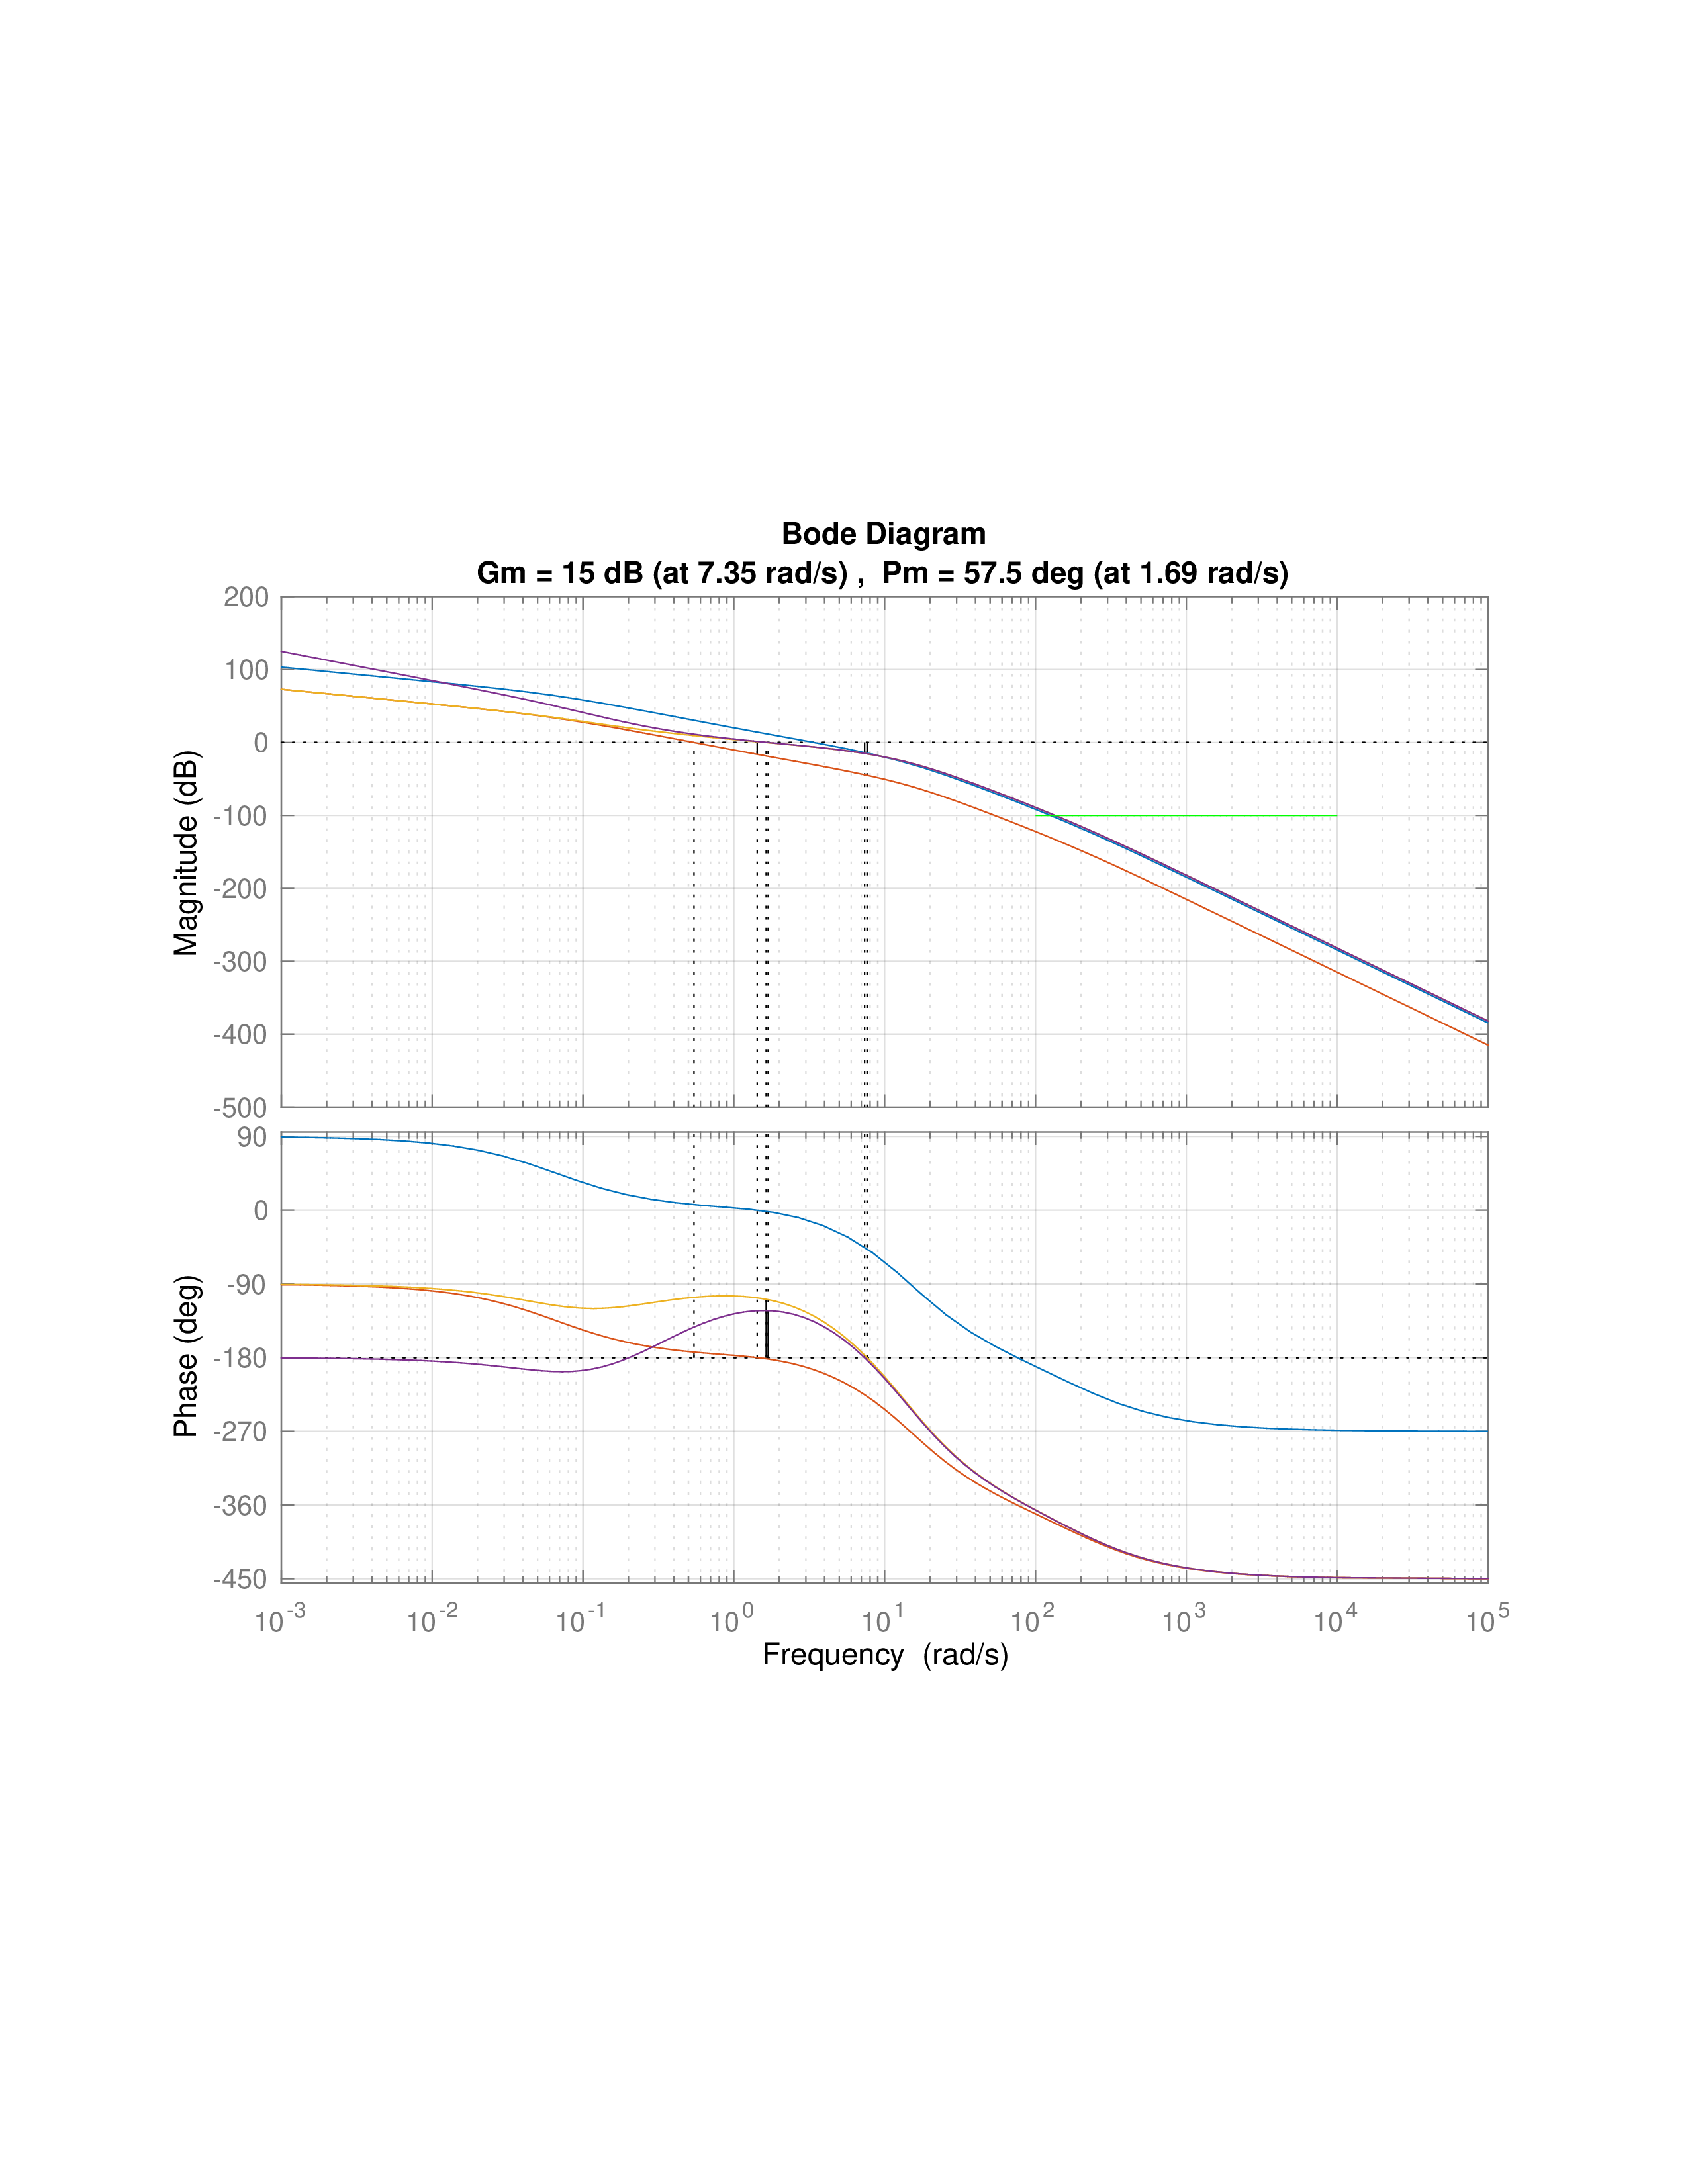
\includegraphics[width=0.95\textwidth]{6_design_studies/figures/hw_vtol_lat_out_compensator_design_4.pdf}
   \caption{The Bode plot for the outer loop of the lateral system in HW~\ref{hw:vtol}.\ref{chap:loopshaping_design} with proportional gain, phase lead, and integral control.}
   \label{fig:hw_vtol_lat_out_compensator_design_4}
\end{figure}

To meet the spec on noise attenuation, the low pass filter
\[
C_{lpf} = \frac{20}{s+20}
\]
and the result is shown in Figure~\ref{fig:hw_vtol_lat_out_compensator_design_5}.
\begin{figure}[H]
   \centering
   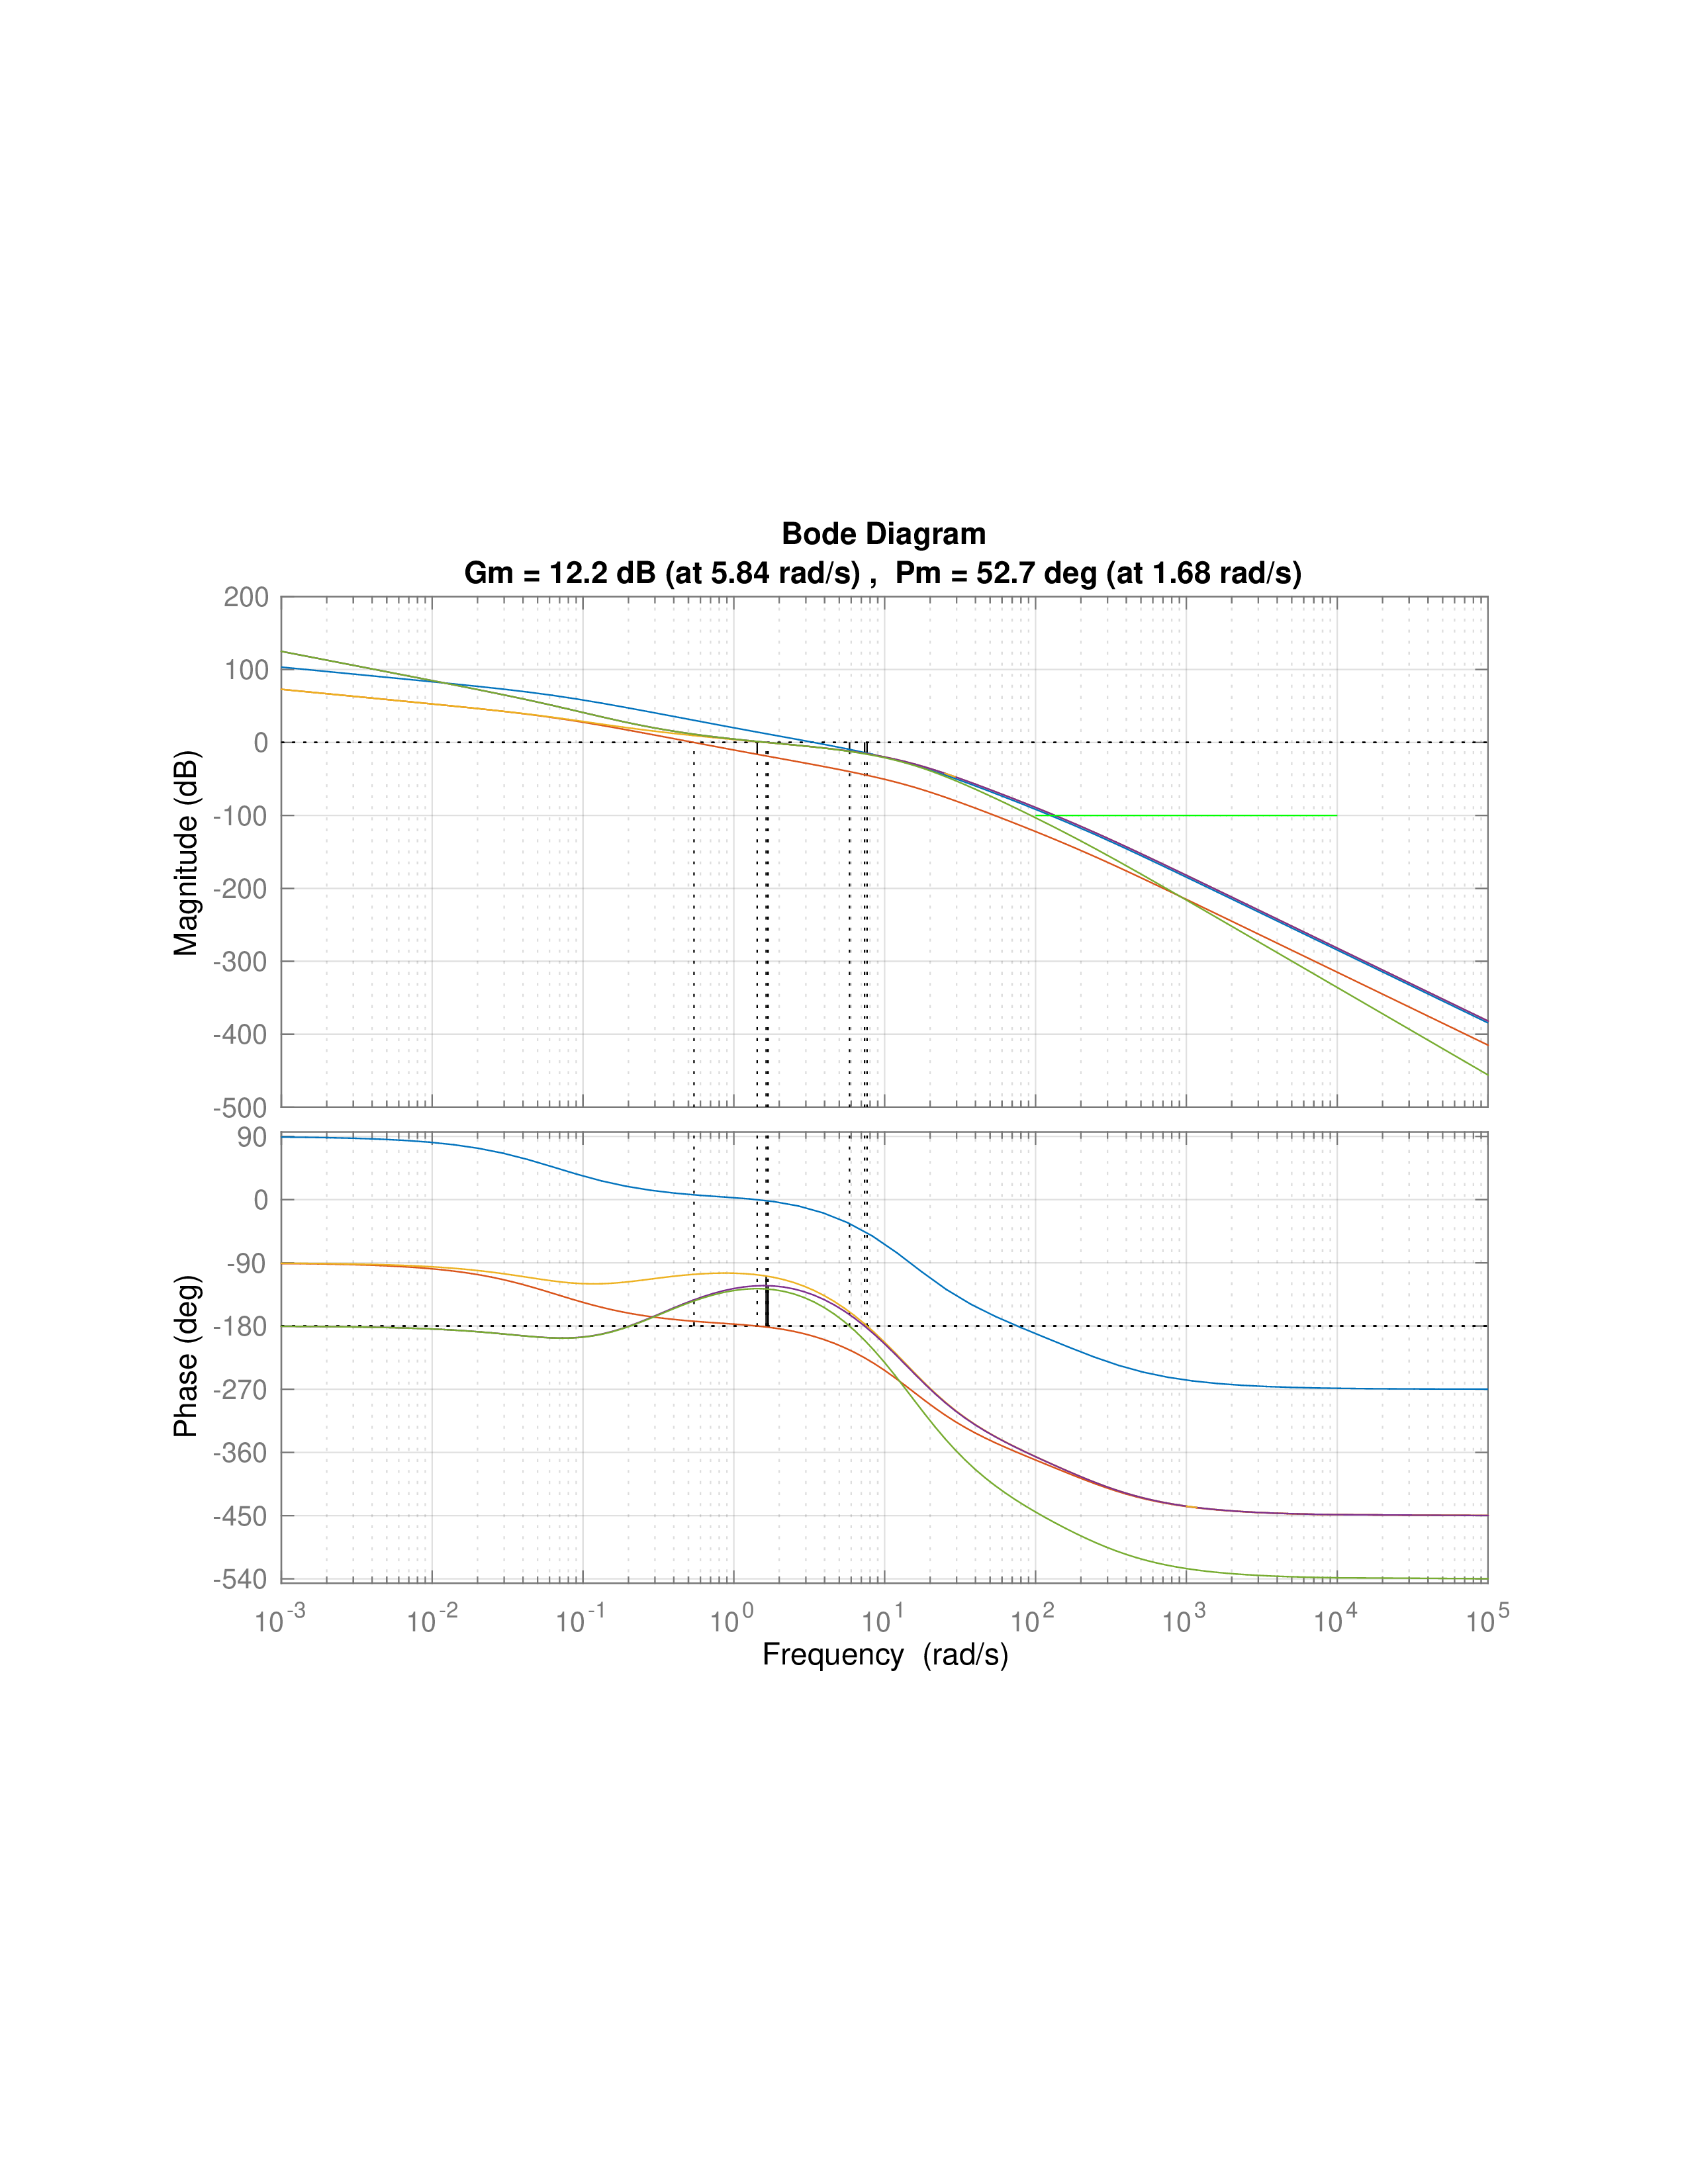
\includegraphics[width=0.95\textwidth]{6_design_studies/figures/hw_vtol_lat_out_compensator_design_5.pdf}
   \caption{The Bode plot for the outer loop of the lateral system in HW~\ref{hw:vtol}.\ref{chap:loopshaping_design} with proportional gain, phase lead, integral control, and low pass filter.}
   \label{fig:hw_vtol_lat_out_compensator_design_5}
\end{figure}
Since the phase margin is $PM=52.7$~degrees, we consider the phase margin specification to be satisfied.
The resulting compensator is
\[
C(s) = -0.03\left(\frac{45(s+1.3/\sqrt{45})}{s+1.3\sqrt{45}}\right)\left(\frac{s+0.4}{s}\right)\left(\frac{20}{s+20}\right).
\]
The closed loop response, 
as well as the unit step response for the output and control signal are all show in Figure~\ref{fig:hw_vtol_lat_out_compensator_design_6}, where the prefilter
\[
F(s) = \frac{0.5}{s+0.5}
\]
has been added to reduce the peaking in the closed loop response.
\begin{figure}[H]
   \centering
   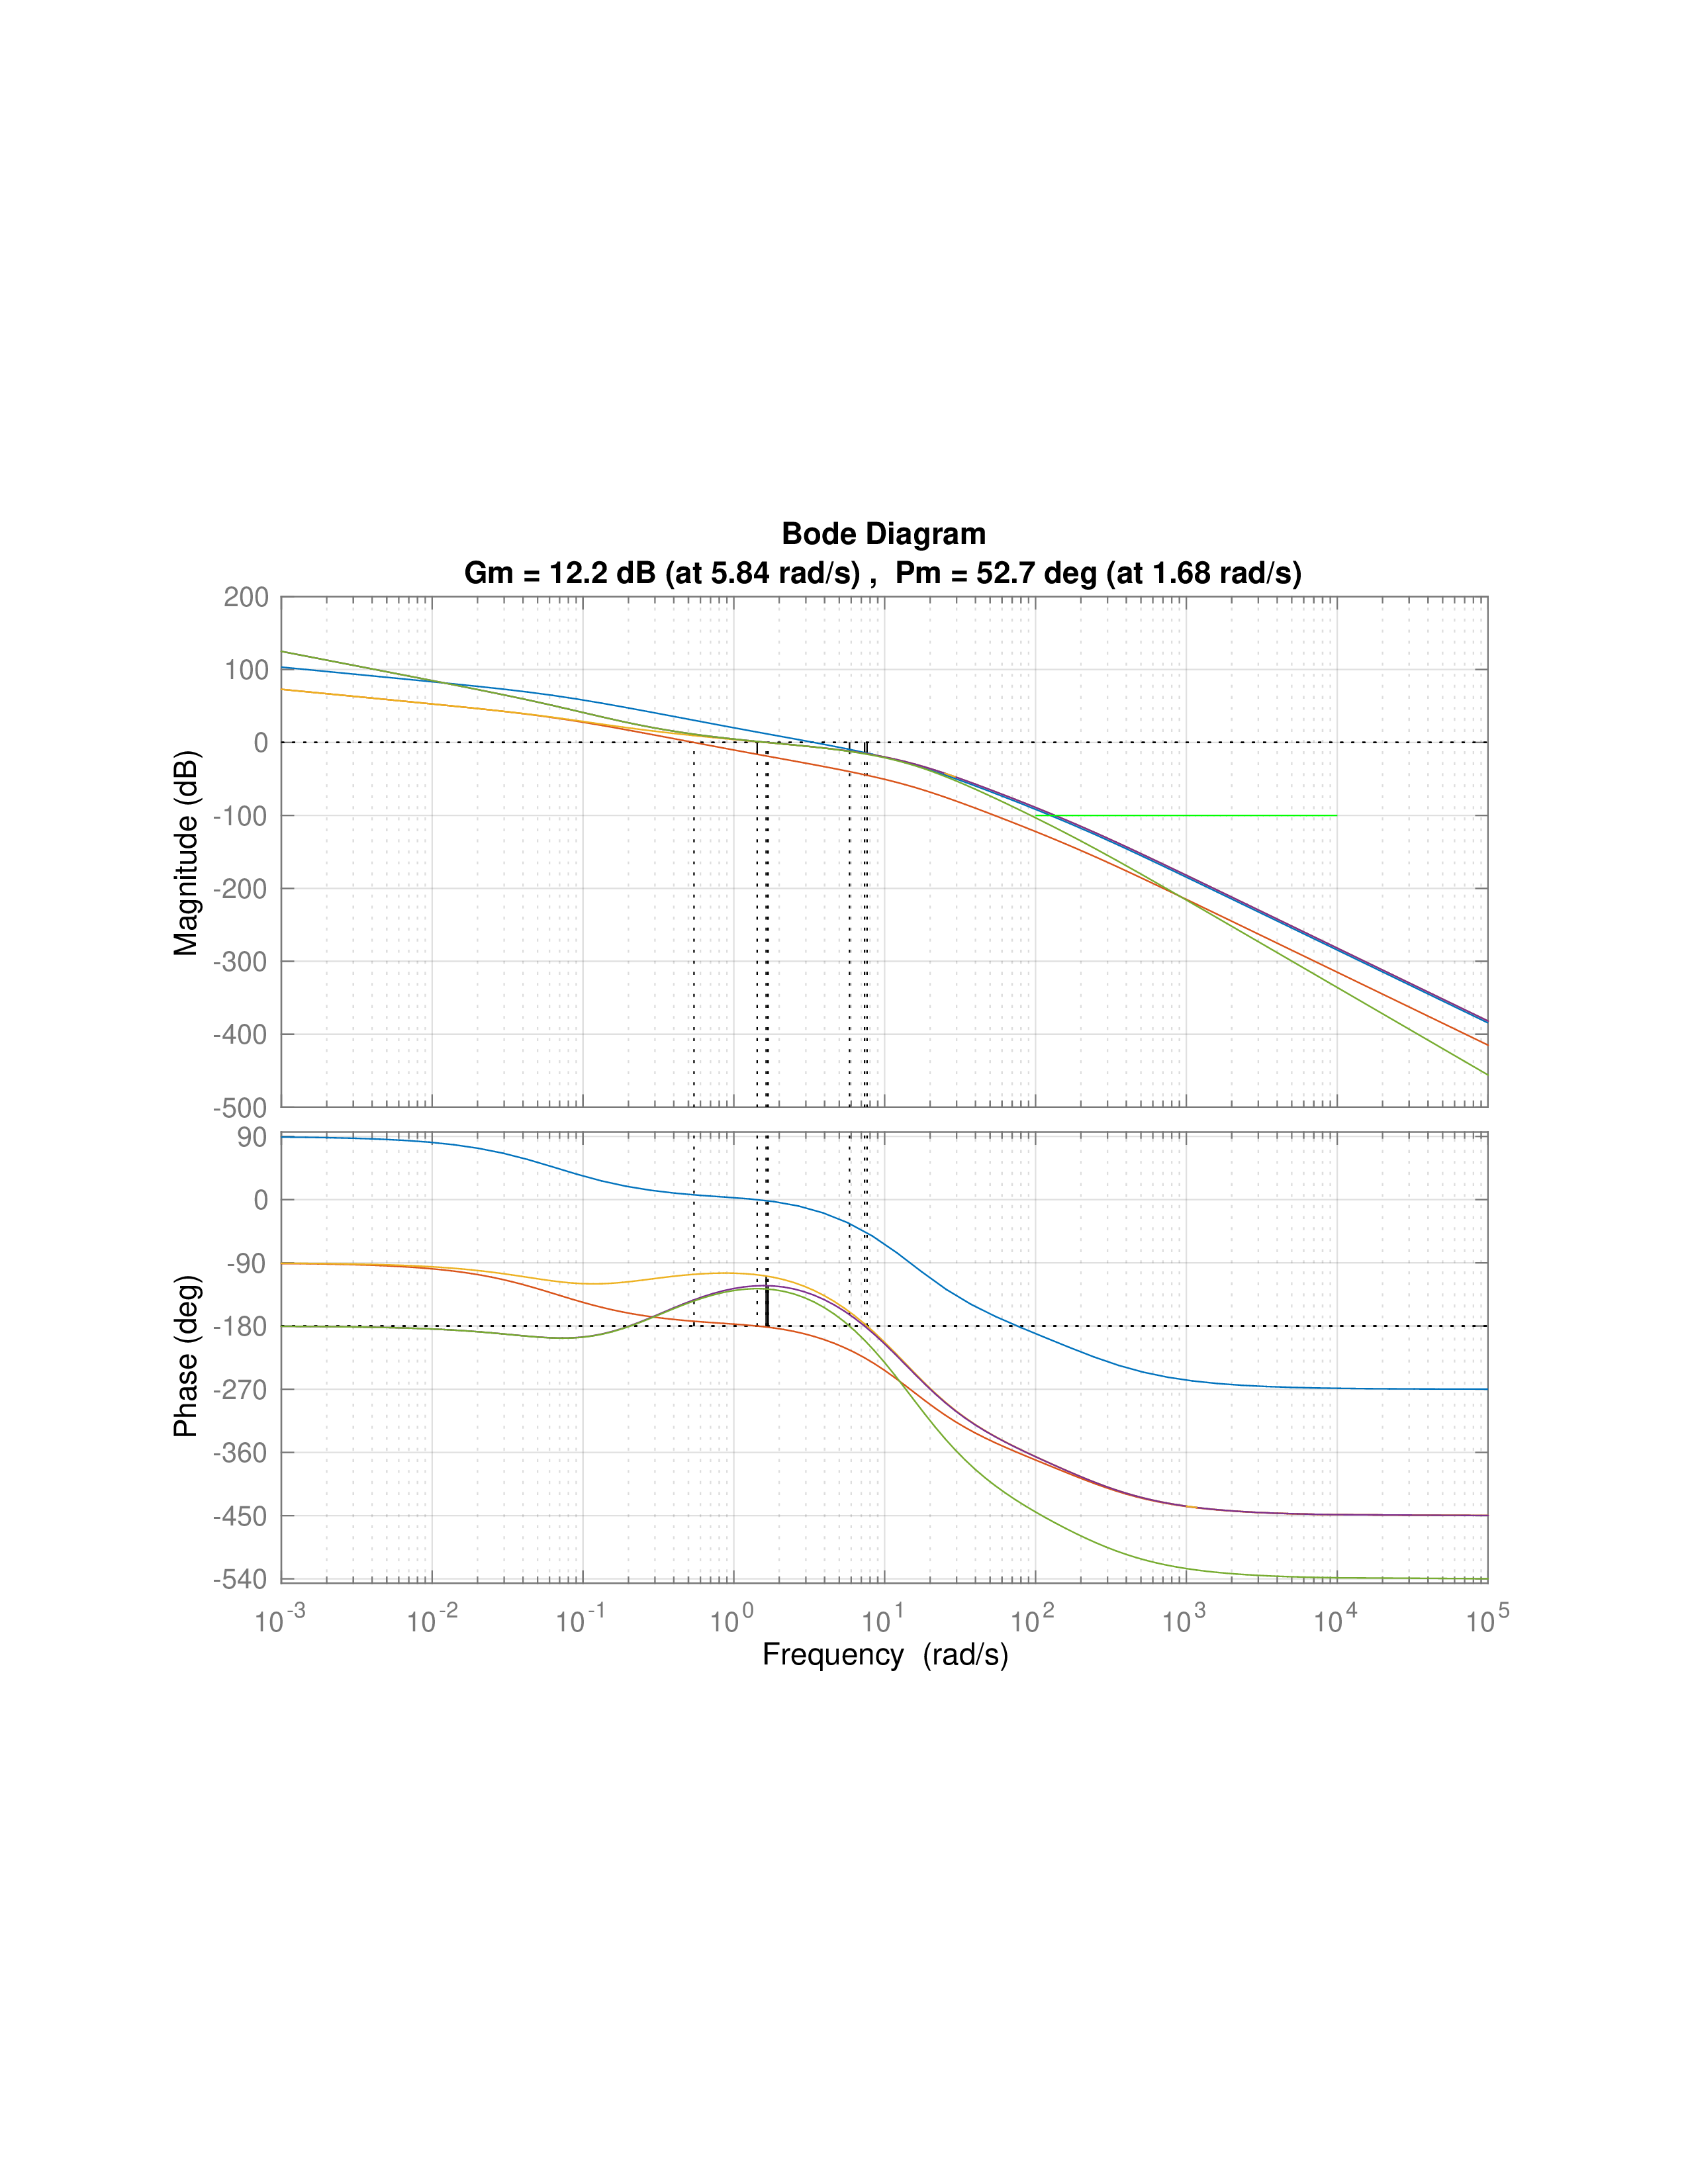
\includegraphics[width=0.95\textwidth]{6_design_studies/figures/hw_vtol_lat_out_compensator_design_5.pdf}
   \caption{The closed loop bode response, the unit step response for the output, and the unit step response for the outer loop of the lateral control for the design in HW~\ref{hw:vtol}.\ref{chap:loopshaping_design}.}
   \label{fig:hw_vtol_lat_out_compensator_design_6}
\end{figure}

The complete solution files are on the wiki associated with the book.



